%%%%%%%%%%%%%%%%%%%%%%%%%%%%%%%%%%%%%%%%%%%
% Template for Doctoral Theses at Uppsala %
% University. The template is based on    %
% the layout and typography used for      %
% dissertations in the Acta Universitatis %
% Upsaliensis series                      %
% Ver 4.0.1 - 2008-11-03                  %
%                                         %
% Publishing & Graphic Services           %
% espik@ub.uu.se                          %
%                                         %
%%%%%%%%%%%%%%%%%%%%%%%%%%%%%%%%%%%%%%%%%%%


\documentclass[11pt,a4paper,twoside, openright]{book} % Default font 11pt, A4, all pages are printed the same, new chapter always begins on a right-hand page.

% Package import
% Language, diacritics and hyphenation
\usepackage[swedish,english]{babel} % Use English and Swedish languages. English default. English hyphenation.
\usepackage[latin1]{inputenc} % Unix users should include this package instead of ansinew or applemac for correct handling of diacritics.
%\usepackage[applemac]{inputenc} % Macintosh users should include this package instead of ansinew or latin1 for correct handling of diacritics.
%\usepackage[ansinew]{inputenc} % % Windows users should include this package instead of applemac or latin1 for correct handling of diacritics.
\usepackage[T1]{fontenc}% Enables the use of 8-bit characters and �, �, � can be typed as �, �, � instead of the corresponding commands.

% Page elements
\usepackage{mathptmx} % Default font for dissertations is Times.
%\usepackage{times} % Default font for dissertations is Times.
%\usepackage{fourier} % If mathematics don't display well using Times, then use Fourier.
%\usepackage{helvet} % Default sans-serif font.
%\usepackage{courier}% Default typewriter (monotype) font.
\usepackage[OT2,OT1]{fontenc}
\def\Sha{{\fontencoding{OT2}\selectfont SH}}

%\usepackage{mathpazo}
\usepackage{Thesis} % This package is specific for theses written at Uppsala University. Modifications to the classfile and the document can be found here.
\ifpdf
   \usepackage[pdftex]{graphicx}
  \else
    \usepackage[dvips]{graphicx}
\fi % Used for figures
\usepackage{booktabs} % Produces good three line tables which is the standard tabel format for disserations.

%\usepackage{mathpazo}
%\usepackage{mathrsfs}
\usepackage{amsmath}
\usepackage{amssymb}
%\usepackage{euler}
\usepackage{eucal}
% This gives me a reasonable looking mathscr font for fourier transforms
\DeclareMathAlphabet{\mathscr}{OMS}{pzc}%
                                 {m}{it}
\usepackage{float}
\usepackage[colorlinks=true, urlcolor=black, pagecolor=black, linkcolor=black,
citecolor=black, filecolor=black, menucolor=black,
pdfpagelabels,bookmarksnumbered=true,plainpages=false]{hyperref} % Use this package to produce
                               % links in the electronic version of the
                               % document. All hyperlinks are black. Page view
                               % is set to Fit Width and page layout is set to
                               % display the document spread.  Make page
                               % anchors using the formatted form of the page
                               % number.  Set PDF page labels; i.e., write the
                               % value of \thepage to the PDF file so that
                               % Acrobat Reader can display the page number as
                               % (say) 'ii (4 of 40)' rather than simply '4 of
                               % 40'.
\usepackage{algorithmic}
\usepackage{algorithm}
\numberwithin{algorithm}{chapter}


% Bibliographic information
% Filling in this bibliographic information facilitates the
% processing of this document.
% Insert linebreaks if necessary
% The abstract page is not generated by default. The reason for this is that it
% will be generated by the unit for Publishing and Graphic sevices from the metadata 
% template ("Spikningsmallen"). If you want to include the abstract page generated from this template,
% please edit the \frontmatterMonograph or \frontmatterCS command at the en of this file
%. Because of this, some of the bibliografic data on this page will not be used.

% Abstract and titelpage
\newcommand{\authorSurname}{Maia} % Your surname
\newcommand{\authorFirstName}{Filipe} % Your given name
\newcommand{\authorFirstInitial}{RNC} % Initial of given name
\newcommand{\authorEmail}{filipe@xray.bmc.uu.se} % Your e-mail address
\newcommand{\dissertationTitle}{Ultrafast Coherent X-ray Diffractive Nano-Imaging} % The title of the dissertation
\newcommand{\dissertationSubtitle}{}% The subtitle of the dissertation (if there is any).
\newcommand{\yearOfPublication}{2010} % Year of publication
\newcommand{\placeOfDisputation}{B41, BMC, Husargatan 3, Uppsala} % Place of disputation
\newcommand{\dateOfDisputation}{Friday, May 14, 2010} % Date of disputation (Day, Month, Year)
\newcommand{\timeOfDisputation}{13:15} % Time of disputation (Swedish time format)
\newcommand{\disputationLanguage}{English} % Language the examination will be conducted in.
\newcommand{\numberOfPages}{51} % The page number of the last page
\newcommand{\placeOfPublication}{Uppsala} % The place of publication
\newcommand{\ISBN}{} % The ISBN number of the dissertation.
%\newcommand{\series}{Uppsala Dissertations from the Faculty of Science and
%  Technology} % The title of the series
\newcommand{\series}{Digital Comprehensive Summaries of Uppsala Dissertations from the Faculty of Science and Technology} % The title of the series
\newcommand{\serialNumber}{} % The number in the series.
\newcommand{\keywords}{free-electron laser, X-ray diffraction, Coherent
  Diffractive Imaging, Image Reconstruction, Single Particle Imaging, keyword6,\\ keyword7, keyword8, keyword9, keyword10,...} % Key words separated by comma
\newcommand{\department}{Department of Cell and Molecular Biology} % Name of your department
\newcommand{\departmentaddress}{Box 596, Uppsala University, SE-75124 Uppsala,
Sweden} % Address of your department
\newcommand{\ISSN}{} % (ISSN for Digital comprehensive summaries of Uppsala dissertations from the faculty of science and technology)
\newcommand{\urn}{urn:nbn:se:uu:diva-} % URN number

% List of papers
\newcommand{\listofpapers}
{\cleardoublepage
\pdfbookmark[0]{List of Publications}{LOP}
\chapter*{List of Publications}
\noindent 
\noindent This thesis is based on the following papers, which are referred
to in the text by their Roman numerals.
\vspace{1\baselineskip}

        % It is possible to refer to the published papers using labels in the text.
        % Suggested order
        % Author 1 surname, Author 2 first name initial., Author 1 surname, Author 2 first name
        % initial. etc. (Year of publication) Paper main title.
        % Paper subtitle. Name of journal in italics, volume(number):page rage
        % Example
        
    \begin{romanlist}


      \item
        \label{cowboys}
        Chapman, H.N., Barty, A., Bogan, M.J., Boutet, S., Frank, M., Hau-Riege, S.P.,
        Marchesini, S., Woods, B.W., Bajt, S., Benner, H., London, R.A., Plonjes, E., Kuhlmann,
        M., Treusch, R., Dusterer, S., Tschentscher, T., Schneider, J.R.,
        Spiller, E., Moller, T., Bostedt, C., Hoener, M., Shapiro, D.A.,
        Hodgson, K.O., Van der Spoel, D., Burmeister, F., Bergh, M., Caleman,
        C., Huldt, G., Seibert, M.M., Maia, F.R.N.C., Lee, R.W., Szoke, A.,
        Timneanu, N., Hajdu J. (2006) Femtosecond diffractive imaging with a
        soft-X-ray free-electron laser. {\em Nature Physics}, 2(12):839-843

    \item
      \label{melting}
      van der Spoel, D., Maia, F.R.N.C., Caleman, C. (2008), Structural studies of
      melting on the picosecond time scale. {\em Physical Chemistry Chemical
        Physics},10(42):6344-6349

    \item 
      \label{music}
      Ravasio, A., Gauthier, D., Maia, F.R.N.C., Billon, M., Caumes, J.P.,
      Garzella, D., Geleoc, M., Gobert, O., Hergott, J.F., Pena, A.M., Perez,
      H., Carre, B., Bourhis, E., Gierak, J., Madouri, A., Mailly, D., Schiedt,
      B., Fajardo, M., Gautier, J., Zeitoun, P., Bucksbaum, P.H., Hajdu, J.,
      Merdji, H. (2009) Single-Shot Diffractive Imaging with a Table-Top
      Femtosecond Soft X-Ray Laser-Harmonics Source. {\em Physical Review
        Letters}, 103:028104

    \item 
      \label{dynamics}
      Maia, F.R.N.C., Ekeberg, T., T\^{i}mneanu, N., van der Spoel, D., Hajdu,
      J. (2009) Structural variability and the incoherent addition of scattered
      intensities in single-particle diffraction. {\em Physical Review E}, 80:031905
      
    \item 
      \label{hawk}
      Maia, F.R.N.C.,  Ekeberg, T., van der Spoel, D., Hajdu, J. (2010)
      Hawk: the image reconstruction package for coherent X-ray diffractive
      imaging. {\em Submitted for publication}
\end{romanlist}

\vspace{1\baselineskip} \noindent {\small Reprints were made with permission from
the publishers.}

\clearpage 

\noindent {\LARGE Supporting Publications}

\vspace{1cm}

\begin{romanlist}
  \setcounter{romanlistc}{5}
\item Bergh, M., Huldt, G., Timneanu, N., Maia, F.R.N.C., Hajdu, J. (2008)
  Feasibility of imaging living cells at subnanometer resolutions by ultrafast
  X-ray diffraction. {\em Quarterly Reviews of Biophysics}, 41(3-4):181-204
  \label{QRB}
\item Bogan, M.J., Benner, W.H., Boutet, S., Rohner, U., Frank, M., Barty, A.,
  Seibert, M.M., Maia, F., Marchesini, S., Bajt, S., Woods, B., Riot, V.,
  Hau-Riege, S.P., Svenda, M., Marklund, E., Spiller, E., Hajdu, J., Chapman,
  H.N. (2008) Single particle X-ray diffractive imaging. {\em Nano Letters},
  8(1):310-316
  \label{nano}
\end{romanlist}
}


% Dedication. Dedication is optional. You can enter whatever feels right and use the fonts and images you like as long as they are embedded in the document. The suggested format does not have to be used.
\newcommand{\dedication}%
{\cleardoublepage
\thispagestyle{empty}
\vspace*{\stretch{3}}
\begin{flushright}
		
{\fontfamily{pzc}\Large\selectfont\emph{to my grandparents...}}

\end{flushright}
\vspace*{\stretch{1}}} % 

% Frontmatter commands
% Halftitle page for monographs
\newcommand{\halftitlepage}{%
\thispagestyle{empty}
\begin{center}
	ACTA UNIVERSITATIS UPSALIENSIS

	\emph{\series{}}
	
	\serialNumber
\end{center}
\cleardoublepage}

% Title page for monographs
\newcommand{\thetitlepage}%
{\thispagestyle{empty}
\vspace*{40mm}
\begin{center}
\Large \authorFirstName{} \authorSurname{}

\vspace{6mm}

\Huge{ \dissertationTitle{}}

\vspace{6mm}

\fontsize{14}{16}\fontshape{it}\selectfont\dissertationSubtitle{}			
\end{center}
\begin{figure}[b]
\begin{center}
\ifpdf

\includegraphics{UU_logo_pc_sv_42}
\else

\includegraphics{UU_logo_pc_sv_42.eps}
\fi
\end{center}
\end{figure}}

% Abstract. This is optional. 
\newcommand{\thesisabstract}{%
\begin{abstract}{%
	\newpage
	\thispagestyle{empty}
    \fontsize{9}{11}\selectfont
    \noindent
    \begin{flushleft}{\nohyphens
    Dissertation at Uppsala University to be publicly examined in \placeOfDisputation{}, \dateOfDisputation{} at \timeOfDisputation{}
    for the Degree of Doctor of Philosophy. The examination will be conducted in \disputationLanguage{}}\end{flushleft}

    \noindent\textbf{Abstract}
    \vspace{-9pt}
    \begin{flushleft}{\nohyphens\noindent\authorSurname{}, \authorFirstInitial{}. \yearOfPublication{}.
    \dissertationTitle{}. \dissertationSubtitle{}. Acta Universitatis
    Upsaliensis. \emph{\series{}} \serialNumber{}. \numberOfPages{}~pp.
    \placeOfPublication{}. ISBN~\ISBN{}}\end{flushleft}

% Type your abstracttext here. Remove the latin text. Try to not type more than 300 words.
\noindent 
% The advent of X-ray lasers provides the scientific community with a
% new kind of instrument that is many orders of magnitude brigther, faster and
% more coherent that existing X-ray light sources. Such revolutionary  change is
% almost certain to be accompanied by a range of new experiments that were
% previously unfeasible.

% One important class of such experiments is ultrafast coherent X-ray diffractive
% imaging (CXDI). In such an experiment an extremely bright and very fast X-ray pulse is
% focused on a sample. The sample is quickly vaporized, but not before scattering
% sufficient light for a diffraction pattern to be recorded. The pattern can then
% be phased and the structure of the undamaged sample recovered.

% This thesis presents the results of some of the first ultrafast X-ray diffractive imaging experiments
% are presented. It combines experiments made using both linear accelerator-driven
% free-electron lasers, and optically driven table-top X-ray lasers. It also
% theoretically explores the possibility of investigating phase transitions in
% crystals using X-ray lasers.

% An important problem with ultrafast CXDI of small samples such as proteins is
% that the signal from a measurement is very small, making the pattern
% uninterpretable. So averaging over multiple equivalent samples will be
% necessary. We present a numerical investigation of the problems introduced when
% the samples are not exactly identical and propose some tentative solutions.

% Hawk, a software package for processing and reconstruction of patterns
% obtained in CXDI experiments is introduced. Currently there is no publicly
% available software for this purpose and we hope Hawk fills this gap. It is
% essential that the rapid progresses in terms of experimental hardware are
% accompanied by equivalent developments on the software side otherwise soon we
% will have much more data that what can be analyzed, and Hawk is released as open
% source with the aspiration of fostering such development.
X-ray lasers are creating unprecedented research opportunities in physics,
chemistry and biology. The peak brightness of these lasers exceeds present
synchrotrons by $10^{10}$, the coherence degeneracy parameters exceed
synchrotrons by $10^9$, and the time resolution is $10^5$ times better. In the
duration of a single flash, the beam focused to a micron-sized spot has the same
power density as all the sunlight hitting the Earth, focused to a millimetre
square. 



Ultrafast coherent X-ray diffractive imaging (CXDI) with X-ray lasers exploits
these unique properties of X-ray lasers to obtain high-resolution structures for
non-crystalline biological (and other) objects. In such an experiment, the
sample is quickly vaporised, but not before sufficient scattered light can be
recorded. The continuous diffraction pattern can then be phased and the
structure of a more or less undamaged sample recovered (speed of light vs. speed
of a shock wave). 



This thesis presents results from the first ultrafast X-ray diffractive imaging
experiments with linear accelerator-driven free-electron lasers and from
optically-driven table-top X-ray lasers. It also explores the possibility of
investigating phase transitions in crystals by X-ray lasers. 



An important problem with ultrafast CXDI of small samples such as single protein
molecules is that the signal from a single measurement will be small, requiring
signal enhancement by averaging over multiple equivalent samples. We present a
numerical investigation of the problems, including the case where sample
molecules are not exactly identical, and propose tentative solutions. 



A new software package (HAWK) has been developed for data processing and image
reconstruction. HAWK is the first publicly available software package in this
area, and it is released as an open source software with the aspiration of
fostering the development of this field.

    \vspace{11pt}

    \noindent
    \emph{Keywords: XFEL, Diffractive Imaging, Single Particle Imaging, X-ray
      Diffraction, X-ray laser, Phasing, Nanoimaging, Ultrafast Imaging}\keywords

    \vspace{11pt}

    \noindent
    \emph{\authorFirstName{} \authorSurname{}, \department{}, Uppsala University,
    \departmentaddress{}}

    \vspace{11pt}

    \noindent \copyright{} \authorFirstName{} \authorSurname{}
    \yearOfPublication{}

    \vspace{11pt}
    
    \noindent ISSN \ISSN{}

    \noindent ISBN \ISBN{}

    \noindent \urn{} (http://urn.kb.se/resolve?urn=\urn)}\end{abstract}}

% Title page dummy for Compehensive summaries
\newcommand{\titlepagedummy}%
{\newpage
\newpage\thispagestyle{empty}
{\noindent\LARGE Titlepage}\vspace{84pt}

\noindent This is the title page dummy. This page should be substituted for a real title page. The real title page will be provided by Publishing and Graphic services after having submitted your posting details in DiVA. The DiVA registration form can be found at \\ \href{https://uu.diva-portal.org/dream/}{https://uu.diva-portal.org/dream/}.

\vspace{1em}

\noindent More information about the publishing routines can be found at \\
\href{http://beta.ub.uu.se/pgs}{http://beta.ub.uu.se/pgs}}

%Abstractdummy
\newcommand{\abstractdummy}%
{\newpage\thispagestyle{empty}
{\noindent\LARGE Abstract page}\vspace{84pt}

\noindent This is the abstract dummy. This page should be substituted for real abstract/imprint page. The real abstract page will be provided by Publishing and Graphic services after having submitted your posting details in DiVA. The DiVA registration form can be found at \\ \href{https://uu.diva-portal.org/dream/}{https://uu.diva-portal.org/dream/}.
\vspace{1em}

\noindent More information about the publishing routines can be found at \\
\href{http://beta.ub.uu.se/pgs}{http://beta.ub.uu.se/pgs}}

% Front matter commands
\newcommand{\frontmatterMonograph}%
{\halftitlepage\thetitlepage\abstractdummy\dedication}

\newcommand{\frontmatterCS}%
{\titlepagedummy\abstractdummy\dedication\listofpapers}
%%% Local Variables: 
%%% mode: latex
%%% TeX-master: "Thesis"
%%% End: 
 % This file should be edited by the author.

\begin{document}
\frontmatter
    %\frontmatterMonograph % Monograph authors use this front matter 
    \frontmatterCS % Authors of Comprehensive Summaries use this front matter 
    % Creates the front matter (title page(s), abstract, list of papers)
    % for either a Comprehensive Summary or a Monograph.
    
    \tableofcontents

    \chapter*{Abbreviations}\label{sec:abrv}

\begin{tabular}{ll}
%EOS     &Electro Optic Sampling\\
%ESI     &Electrospray Ionization\\
CXDI    &Coherent X-ray Diffraction Imaging\\
FEL     &Free Electron Laser\\
FFT     &Fast Fourier Transform\\
FLASH   &Free Electron Laser in Hamburg\\
fs      &femtosecond\\
%GROMACS &Groningen Machine for Chemical Simulations\\
HIO     &Hybrid-Input Output\\
%IR      &Infra Red\\
LCLS    &Linac Coherent Light Source\\
%LJ      &Lennard-Jones\\
%MD      &Molecular Dynamics\\
%MM      &Molecular Mechanic\\
%MS      &Mass Spectroscopy\\
%NMR     &Nuclear Magnetic Resonance Spectroscopy\\
%PBC     &Periodic Boundary Conditions\\
%PME     &Particle-mesh Ewald\\
%PPPM    &Particle-Particle Particle-Mesh\\
%QM      &Quantum Mechanic\\
PRTF    &Phase Retreival Transfer Function\\
RAAR    &Relaxed Averaging Alternating Reflection\\
SASE    &Self Amplified Spontaneous Emission\\  
SCSS    &Spring-8 Compact Sase Source\\
SLAC    &Stanford Linear Accelerator Center\\
%SPC     &Single Point Charge\\
%SPPS    &Sub Pico-second Pulse Source\\
%TPP     &Tanuma, Powell and Penn\\
%TTF     &Tesla Test Facility\\
VUV     &Vacuum Ultra Violet\\
XFEL    &X-ray Free Electron Laser
%Atomic	&Laser orbital\\
%BO	&Born - Oppenheimmer\\
%CI	&Configuration Interaction\\
%CPMD	&Car-Parinello Molecular Dynamics\\
%DFT &Density Functional Theory\\
%DNA &Deoxyribose Nucleic Acid\\
%FO &Frontier Orbital\\
%GC &Gradient Corrected\\
%GGA &Generalised Gradient Approximation. Synonymous to GC.\\
%HF &Hartree - Fock\\
%HK &Hohenberg - Kohn\\
%IEF-PCM &Integral Equation Formalism - PCM. See PCM below.\\
%KS &Kohn - Sham\\
%LDA &Local Density Approximation\\
%LSDA &Local Spin Density Approximation\\
%MO &Molecular Orbital\\
%MO-LCAO &MOs as Linear Combinations of Atomic Orbitals\\
%NMR &Nuclear Magnetic Resonance\\
%PC &Product Complex\\
%PCM &Polarisable Continuum Model\\
%PES &Potential Energy Surface\\
%RC &Reactant Complex\\
%RHF &Restricted Hartree - Fock\\
%SAR	&Structure - Activity Relationships\\
%SCF &Self Consistent Field\\
%TS &Transition State\\
\end{tabular}
'

    % Optional tables
    %\listoftables
    %\listoffigures

\mainmatter
    % This includes the "Instruction", "Problem and Solutions" and "Example"
    % files. After reading it, remove it from Thesis.tex. 
\chapter{Introduction}\label{introduction}\noindent

Mankind has always had a fascination with looking at the infinitely
small. Since the invention of microscope people have been trying to find ways to
look at smaller and smaller things. The invention of X-ray crystallography in
the beginning of the twentieth century made it possible to observe the
structures of things much smaller than the wavelength of visible light.

Nowadays X-ray crystallography is one of the most successful techniques ever
developed, and every year thousands of new protein structures are solved and deposited
in the Protein Data Bank. It is currently the only technique capable of
delivering atomic resolution images of biological macromolecules which are
invaluable in, for example, the understanding of biology or in the creation of
new drugs. Cryo electron microscopy also shows great promise with current
structures frequently achieving resolutions below 10 \AA, but still not enough
for atomic resolution.

However X-ray crystallography, as the name suggests, is limited to systems that
can be crystallized. Many, if not most, systems of biological interest are very
difficult, or impossible to crystallize. Probably the most striking example is
that of a simple cell, but there are many others such as organelles and many
membrane proteins. Alternative approaches have to be employed to image these
samples, including cryo electron microscopy, atomic force microscopy or
transmission electron microscopy. Unfortunately all of these alternatives have
serious drawbacks compared to X-ray crystallography such as not being able to
image the interior of the samples, providing a lower resolution or requiring
extensive sample preparation which might potential alter it.

Ultrafast Coherent X-ray Diffractive Imaging(CXDI) is a relatively new
technique, which uses a coherent, short and extremely
bright pulse of X-rays to capture a diffraction image of the sample which is
then phased to reveal the sample structure, has the potential to allow three
dimensional imaging of non-periodic reproducible biological samples up to atomic
resolution and two dimensional imaging of non reproducible samples up to
very high resolution, without the need of slicing or staining the sample.

CXDI requires extremely a very high number of photons as it does not benefit from the
amplification effect of a crystal as X-ray crystallography does. But on the
other hand it is possible to sample the diffraction pattern in between the Bragg
peaks which makes the phasing problem much simpler. To be able to achieve high
resolution using CXDI very short pulses are necessary otherwise the radiation
damage that develops during the exposure limits the maximum resolution. For
example the highest resolution possible for biological samples using current
synchrotron based x-ray microscopes is around 20nm, limited by radiation damage.

The recent development of X-ray free electron lasers (XFELs) is the perfect
instrument to realize the full potential CXDI. XFELs can produce extremely
intense X-ray pulses, a billion times more brilliant than third
generation synchrotron sources, which are also extremely short, on the order of
only a couple femtoseconds. FLASH, in Hamburg, Germany, was the first soft X-ray
free electron laser in the world, and is based on the Self Amplified Spontaneous
Emission (SASE) principle. It started operations in the summer of 2005 at
a wavelength of 32nm and a peak power on the order of GW and pulse length up to
10fs. It has gone through several updates reaching the wavelength of
6.5nm. Despite being the test facility for the European X-ray Free Electron
Laser it has produced many important results in the CXDI field \cite{Cowboys, Chapman Holography}. In April 2009 the Linac Coherent Light Source (LCLS)
became the first hard X-ray free electron laser in the world producing light
with a wavelength of \mbox{1.5 \AA}. The Sprint-8 Compact SASE Source (SCSS) in
Japan will soon be ready and the European X-ray Free Electron Laser (XFEL)
will follow in a few years.

During the last few years there has also been a rapid development of tabletop
high harmonic generation (HHG) sources. These have the potential to one day
compete with free electron lasers and they are much more affordable for
individual labs. Nowadays there are HHG sources with very good coherence
properties capable of producing extremely short pulses, under 1fs, at soft X-ray wavelengths and more than $10^{11}$ photons
per pulse \cite{Ravasio}. This is still a few orders of magnitude below what is
possible using XFELs but due to the lower cost and greater access they might
become important tools in the near future.

The availability in the near future of several hard XFELs combined with the
increasing development of CXDI experimental techniques and data processing
algorithms have the potential to transform Ultrafast Coherent X-ray Diffractive
Imaging from a niche unconventional technique into a mainstream structural
biology tool that complements X-ray crystallography, as well as a general
imaging method such as electron microscopy.


%I'm pretty sure i need to reformulate this 
The aims of this thesis are: to present recent experimental results in Ultrafast
Coherent X-ray Diffractive Imaging using both free electron lasers and
HHG sources, to theoretically investigate the problem of sample heterogeneity
for reproducible samples and to propose new experiments made possible with this
new sources.
%%% Local Variables: 
%%% mode: latex
%%% TeX-master: "Thesis"
%%% End: 

\chapter{New Ultrashort X-ray Sources}\label{Ultrashort X-ray Sources}\noindent
 
Since the discovery of X-rays by Wilhelm R\"{o}ntgen in 1895 X-ray sources have
continuously improved, often leading to significant new science. The increase in
brilliance since the first rotating anodes used for crystallography has been
spectacular, bridging many orders of magnitude. The development of dedicated
synchrotron light sources in the beggining of the 80s contributed to an explosion of
protein structures solved by crystallography. A further boost came with
the introduction of wigglers undulators and the increase in brightness from
third generation sources.

 
\begin{figure}[h]
\centering
  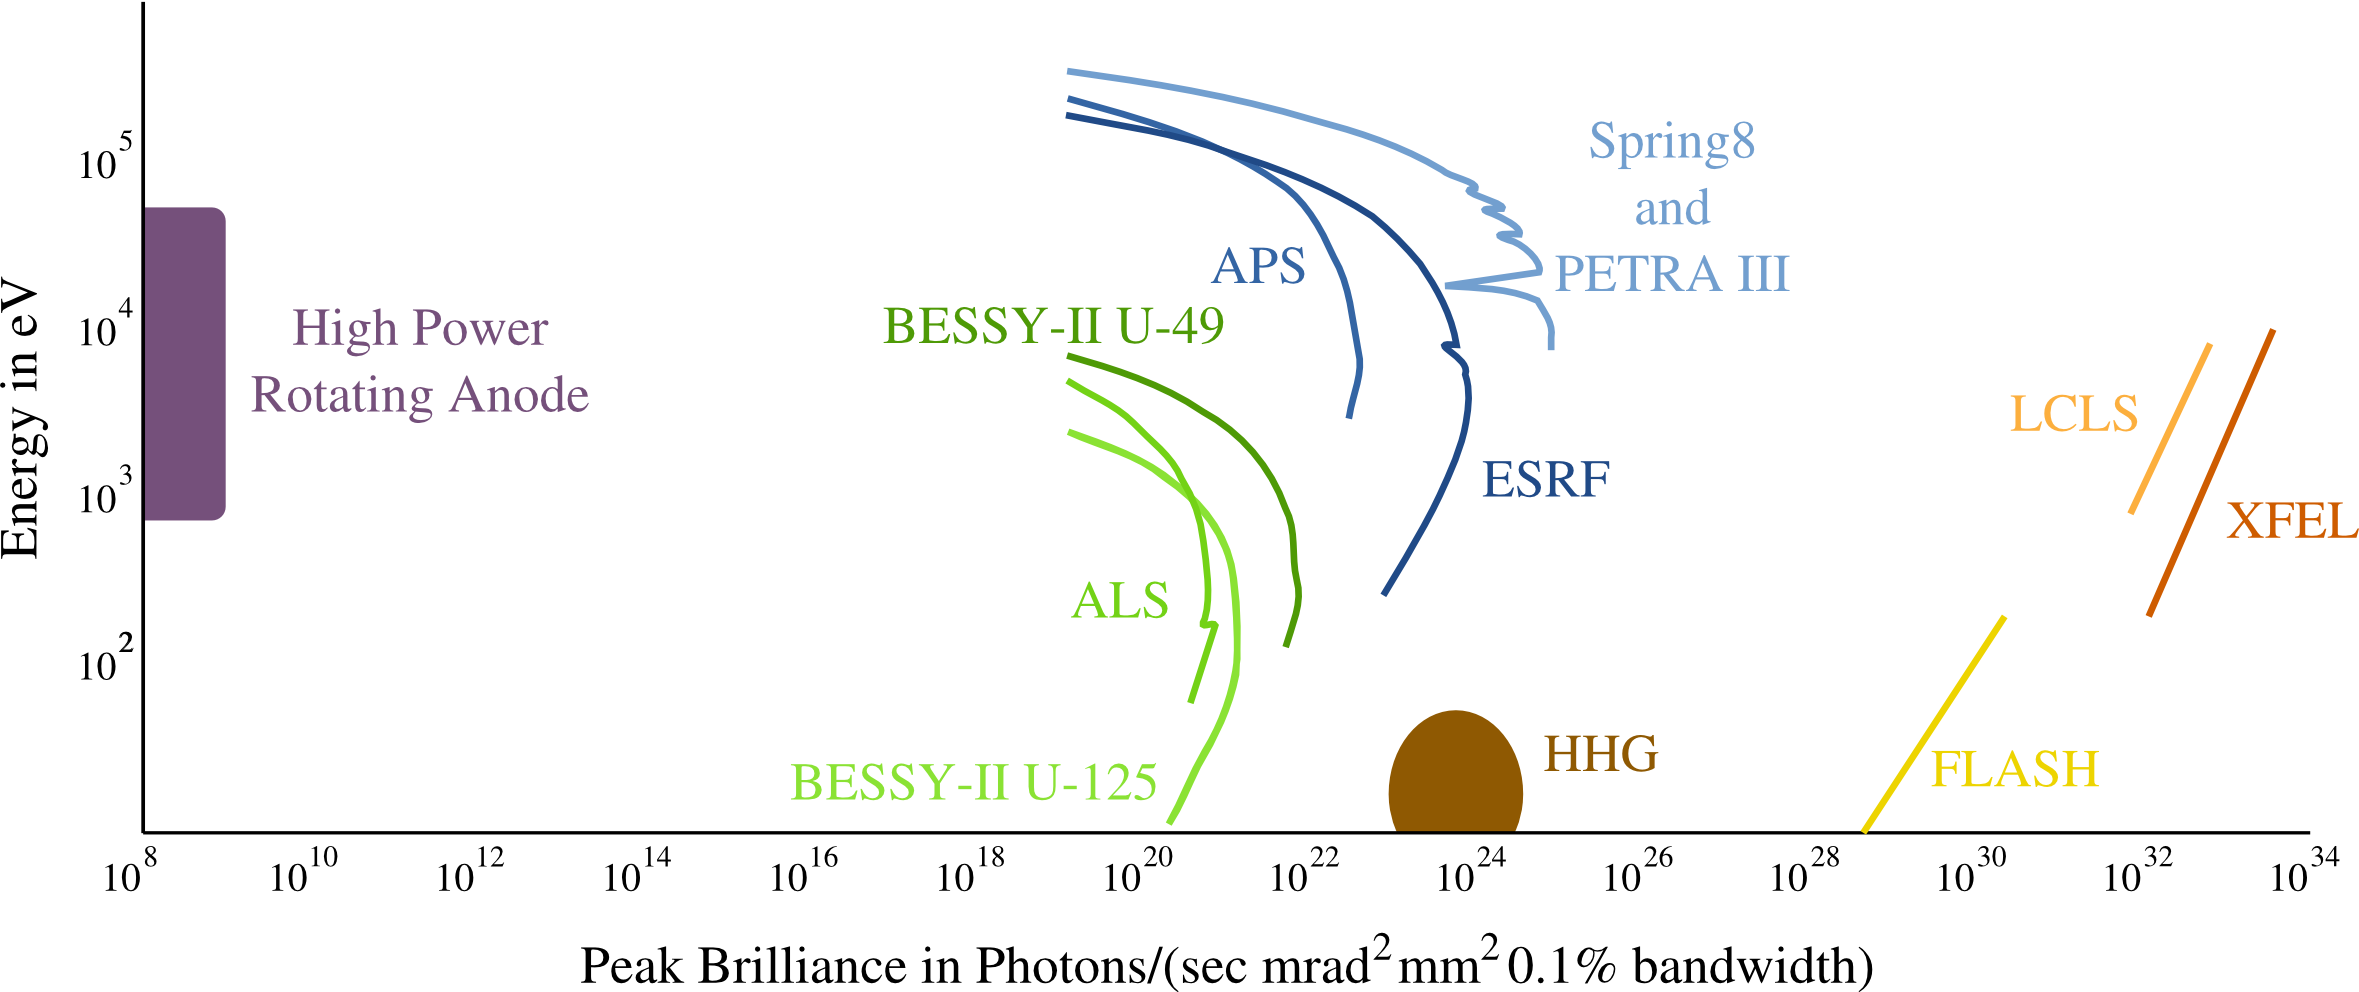
\includegraphics[width=1.0 \columnwidth]{brilliance.png}
  \caption{Peak brilliance of several X-ray sources.}
%    http://www.nature.com/nphoton/journal/v1/n6/abs/nphoton.2007.76.html and TESLA_Technical_design_Report
  \label{Fig:Brilliance}
\end{figure}

The introduction of free electron lasers brings with it an increase in peak
brightness comparable to the change from rotating anodes to synchrotron sources
(Fig. \ref{Fig:Brilliance}). They also offer very high coherence and ultra fast
pulses of only a couple of femtoseconds opening a new window into the world of
ultra fast science. HHG sources also shares many of the characteristics of free
FELs albeit with lower peak power. In this chapter we will try to provide an
overview of these two light sources.

\section{Free electron lasers}

Free electron lasers are in many ways an evolution from third generation
synchrotrons and so they are often called fourth generation light sources. The
fundamental difference between these two light sources is that while in a
synchrotron photons are generated independently of each other in a free electron
laser photon are generated in phase with each other and so cooperate to produce
a pulse which has an intensity proportional to the square of the number of
electrons being accelerated, instead of being linear with the number of
electrons as is the case for a synchrotron.

\subsection{The SASE process}

The SASE process, central to all existing X-ray free electron lasers, is a
process in which the electrons are organized in micro bunches separated by the
distance of a wavelength, as they go through the undulator (see
Fig. \ref{Fig:Brilliance}). This happens because,
as in a normal synchrotron, when the electrons go through the undulator they
will emit radiation due to the acceleration of imposed by the magnetic field. If
the undulator is sufficiently long this radiation will starts to produce a
measurable effect in the distribution of the electrons making them accumulate in
micro bunches separated by exactly one wavelength. This is a self reinforcing
process as the more the electrons bunch together the stronger the field they
produce as they will radiate coherently. This process continues until almost all
the electrons are in these micro-bunches, at which point it is said that
saturation is reached. 

\begin{figure}[h]
\centering
  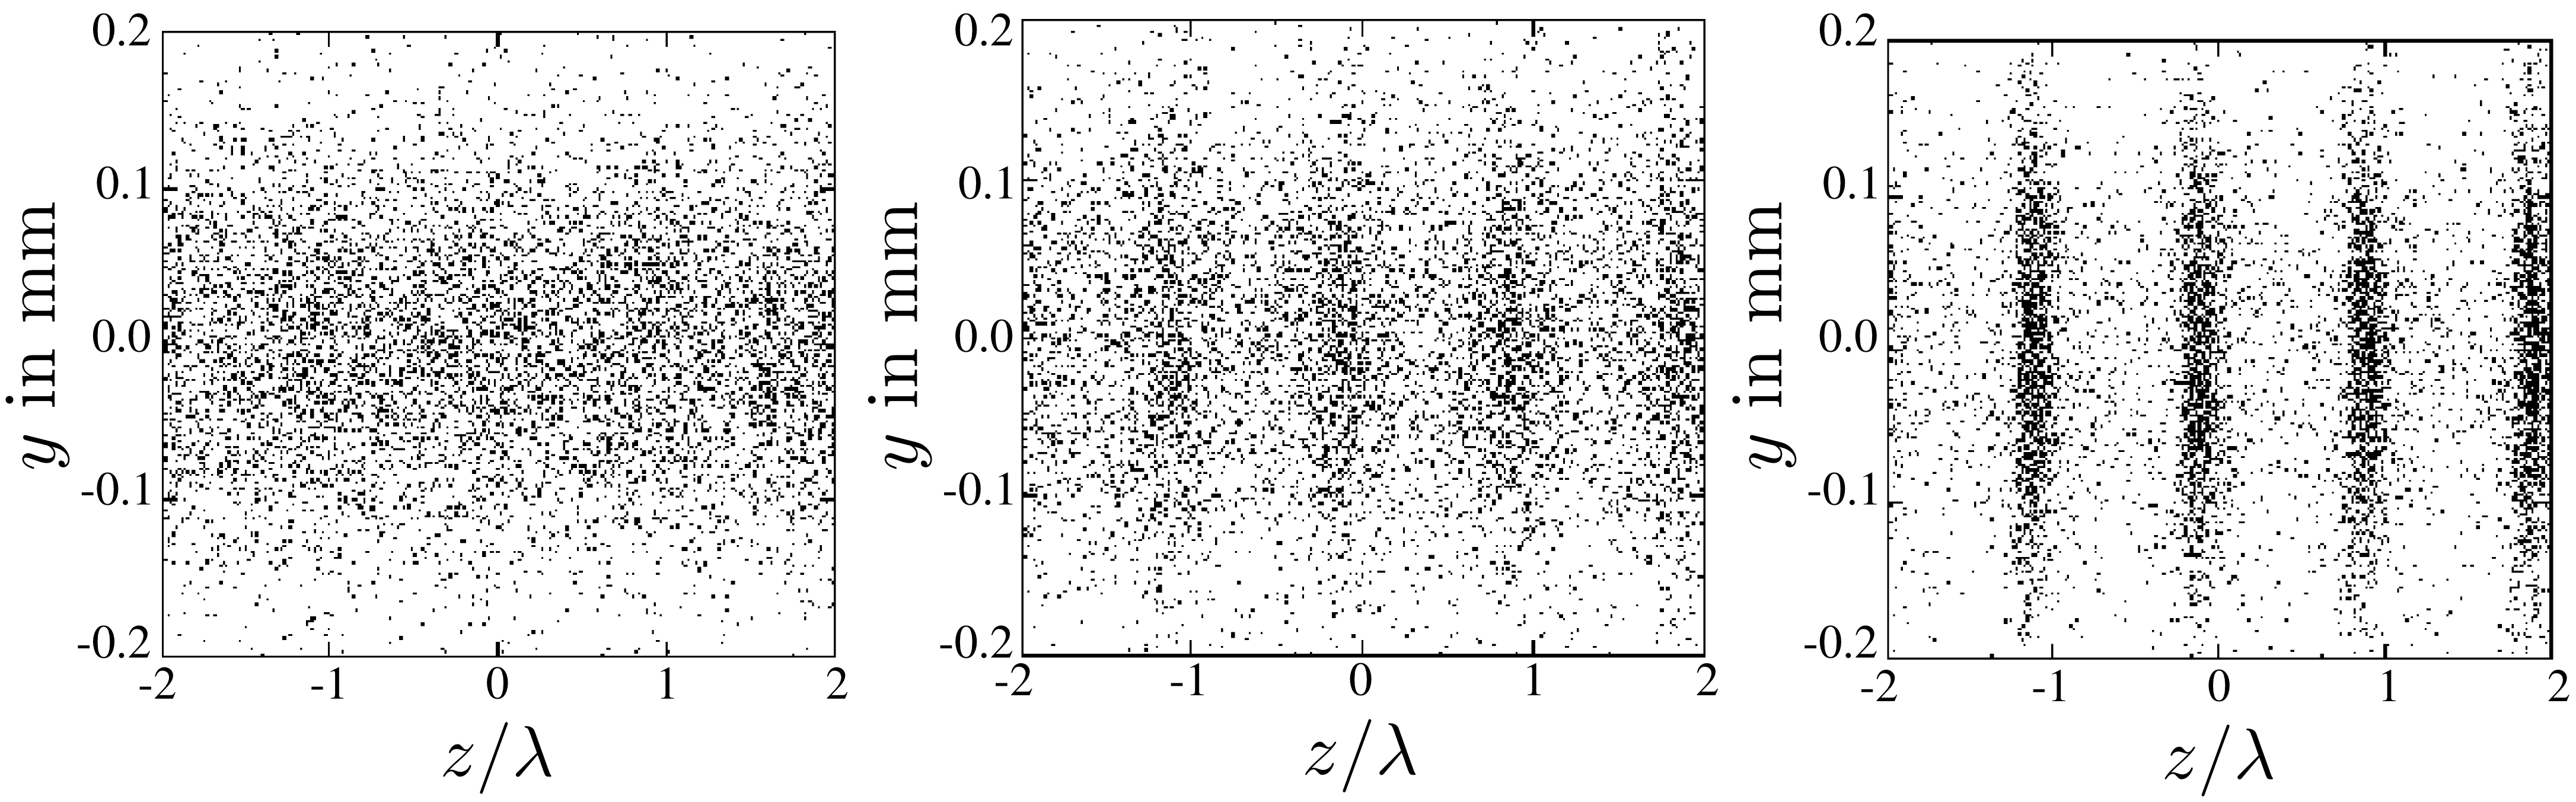
\includegraphics[width=1.0 \columnwidth]{micro-bunching.png}
  \caption{Simulation of micro-bunching during the SASE process where the
    electron density is represented by the density of dots. The snapshots
    from the left to the right represent the electron structure along the
    undulator, with the left side representing the beggining and the right side
    the end of the undulator. \ref{TESLA_Technical_design_Report}}
  \label{Fig:Brilliance}
\end{figure}

The radiation produced by electrons distributed in this manner is much more
intense than if the electrons were uniformly distributed throughout the
undulator because with microbunching the distance between most of the electrons is
always a multiple of the wavelength, and so the radiated electric fields will be
in phase. In other words the electrons radiate coherently and the resulting
intensity will scale will the square of the number of electrons which is why the
difference in peak brilliance is so large.

\subsection{Current X-ray FEL Facilities}

X-ray FEL are developing at a very fast pace. E
Nowadays there is only one hard X-ray FEL facility, LCLS at SLAC, USA and one
one soft X-ray FEL named FLASH in DESY, Germany. But there are several X-ray FEL
being built such as the european XFEL in Germany and SCSS
in Japan both hard X-ray FEL as well as several soft X-ray sources such as FERMI
in Italy. The SwissFEL in Switzerland is also in planning stages. 
Due to the fact that X-ray FEL use linear accelerators it is only
possible to have beam in one beamline at the same time so even though the number
of facilities is increasing quickly, access to an X-ray FEL will continue to be
severely limited. This in combination with the different characteristics of FEL
radiation compared to a third generation synchrotron mean that while they are
often called fourth generation sources they will not replace synchrotrons in any
meaninful sense as it happened in the past. They should be considered a class of
their own better suited for other kinds of experiments not possible at synchrotrons.

\section{High harmonic generation}

The first High harmonic generation (HHG) sources were discovered about two decades ago
and since then their power has been increasing as the power of optical lasers
increases. They provide a relatively cheap source and tunable source of very
short (a few fs) and intense pulses (more than $10^{10}$ photons per pulse). 

HHG works by shining a very intense optical laser in a gas. When the field of
the optical laser is sufficiently strong the electron in the gas will be ionized
by field ionization, and as the field progresses they will be accelerated back
towards the ion and finally recombine, generating in the process short
wavelength radiation (see Fig. \ref{Fig:HHG_Process}).

\begin{figure}[h]
\centering
  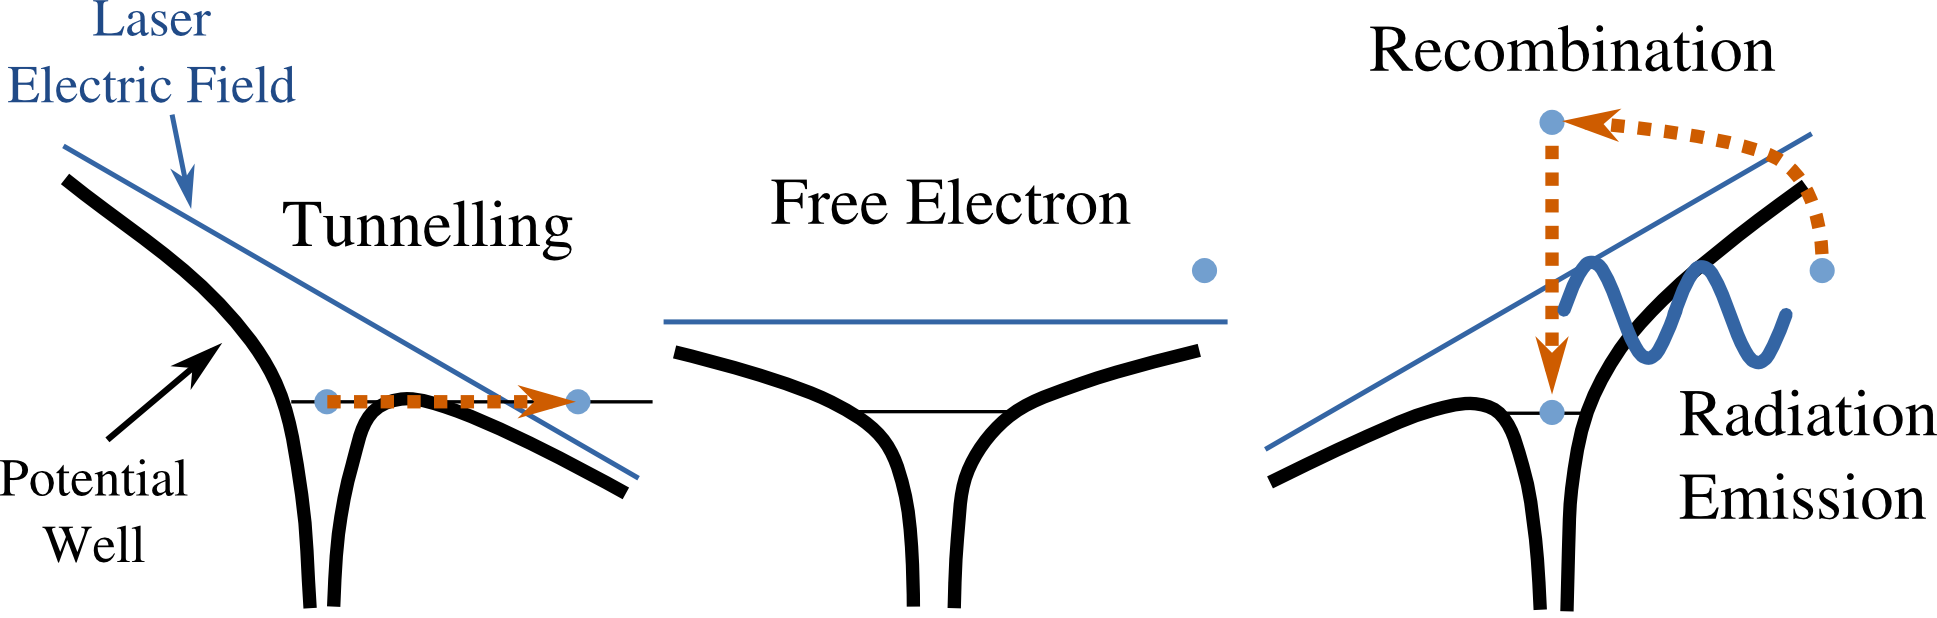
\includegraphics[width=1.0 \columnwidth]{HHG_Picture1.png}
  \caption{High harmonic generation process in an atom iluminated by an intense
    optical laser. The field is strong enough to distort the atomic potential
    well and allowing the electron to tunnel out. When the field reverses the
    electron is accelerated back towards the ion, and recombines generating high
    energy radiation.}
  \label{Fig:HHG_Process}
\end{figure}

% * High Harmonic Generation

% - Started one decade ago
% - Short description with non linear effects
% - Show some scheme of the setup
% - Very short pulse lengths
% - 
%%% Local Variables: 
%%% mode: latex
%%% TeX-master: "Thesis"
%%% End: 

\chapter{An Introduction to Fourier Transforms}\label{fourier_transform_basics}\noindent
Fourier transforms are used extensively in the subject of diffraction and
imaging, so in this chapter we present a basic introduction describing the
Fourier transform and its most commonly used properties. These properties will
be fundamental for both for the description scattering and for the explanation
of image reconstruction algorithms.

\section{Continuous Fourier Transform}

We will start by defining the continuous forward Fourier transform, following crystallographic tradition, as,
\begin{equation}
\hat{f}(q) = \mathscr{F}f = \int \limits_{-\infty}^{\infty} 
f(x) \exp(2 \pi i q \cdot x) \, dx
\end{equation}
and the inverse transform as,
\begin{equation}
f(x) = \mathscr{F}^{-1}\hat{f} = \int \limits_{-\infty}^{\infty} 
\hat{f}(q) \exp(-2 \pi i q \cdot x) \, dq.
\end{equation}
The following properties of the Fourier transform will be important for the rest of the thesis:
%The Fourier transform has the following properties:
\begin{enumerate}
\item The Fourier transform is a linear transformation. For any two complex
  numbers $a$ and $b$,
\begin{equation}
\mathscr{F}\left\{ a f(x) + b g(x)\right\} = a \mathscr{F}f(x) + b \mathscr{F}g(x)
\end{equation}

\item ``Stretching'' a function ``squeezes'' its Fourier  transform,
\begin{equation}
\mathscr{F}\left\{f(a x)\right\} = \frac{1}{|a|}\hat{f}(\frac{x}{a}) 
\end{equation}
where $a$ is a real number different from zero. This is known as the scaling
property or theorem.

\item The Fourier transform of a real function $f(x)$ is a hermitian function,  
\begin{equation}
\hat{f}(q) = \overline{\hat{f}(-q)}
\end{equation}
where $\overline{x}$ represents the complex conjugate of $x$.
\item The Fourier transform of an hermitian function $f(x)$ is a real function,
\begin{equation}
Im\left[\hat{f}(q)\right] = 0
\end{equation}
where $Im\left[x\right]$ represents the imaginary part of $x$.
\item The Fourier transform of a function translated by an amount $\Delta x$ is
  related to the transform of the original function by a factor of $\exp(2 \pi i
  \Delta x q)$ ,
  \begin{equation}
    \mathscr{F} f(x+\Delta x) = \exp(2 \pi i \Delta x q) \mathscr{F} f(x)
\end{equation}

\item The integral of the square of the absolute value of a function and it's Fourier transform are identical
\begin{equation}
\int |\hat{f}(q)|^2 dq = \int |f(x)|^2 dx.
\end{equation}
This is usually known as Parseval's theorem or Rayleigh's energy theorem

\item The convolution of any two functions is equal to the inverse Fourier transform of the product of the forward Fourier transform of those two functions,
\begin{eqnarray}
f(x) * g(x) & = & \int f(\tau) g(x-\tau) \, d\tau \nonumber \\
& = & \mathscr{F}^{-1}\left\{\mathscr{F}f(x) \times \mathscr{F}g(x)\right\}
\end{eqnarray}
where $f(x) * g(x)$ denotes the convolution of $f(x)$ with $g(x)$. This property
is known as the convolution theorem.

\item The cross-correlation of any two functions is equal to the inverse Fourier
  transform of the product of the forward Fourier transform of one function with
  the complex conjugate of the forward Fourier transform of the other function,
\begin{eqnarray}
f(x) \star g(x) & = & \int f(\tau) g(x+\tau) \, d\tau \nonumber \\ 
& = & \mathscr{F}^{-1}\left\{\mathscr{F}f(x) \times \overline{\mathscr{F}g(x)}\right\}
\end{eqnarray}
where $f(x) \star g(x)$ denotes the cross-correlation of $f(x)$ with $g(x)$.
 
\item Finally the correlation of a function with itself, also known as
  autocorrelation is equal to the inverse Fourier transform of the absolute
  value squared of the forward Fourier transform of that function,
  \begin{eqnarray}
f(x) \star f(x) & = & \mathscr{F}^{-1}\left\{\mathscr{F}f(x) 
  \times \overline{\mathscr{F}f(x)}\right\} \nonumber \\
& = & \mathscr{F}^{-1}\left\{|\mathscr{F}f(x)|^2\right\}
\end{eqnarray}
\end{enumerate}

\section{Discrete Fourier Transform}

In practice we will be dealing with signals which are not continuous, but
discrete, as most signal recording is done digitally nowadays and to be able to
perform numerical computations with any input we first need to digitize
it. Fortunately there is a discrete analogue of the Fourier transform called
the discrete Fourier transform (DFT). The one dimensional discrete Fourier
transform of a vector $\mathbf x$ of length N is defined by
\begin{equation}
\hat{\mathbf x}_k = \mathscr{F}\left\{ \mathbf x\right\}_k = \frac{1}{\sqrt{N}} \sum
\limits_{n=0}^{N} \mathbf x_n \exp\left(2 \pi i k \frac{n}{N}\right) \, ,
\end{equation}
and the inverse pair as
\begin{equation}
{\mathbf x}_n = \mathscr{F}^{-1}\left\{ \mathbf x\right\}_n = \frac{1}{\sqrt{M}} \sum
\limits_{k=0}^{M} \hat{\mathbf x}_k \exp\left(-2 \pi i n \frac{k}{M}\right) \, .
\end{equation}

Throughout this thesis we will commit a slight abuse of notation and use
$\mathscr{F}$ to symbolize both the continuous Fourier transform, when the
operand is a function, and the discrete Fourier transform, when the operand is a
vector.
 
The DFT has properties analogous to most properties of its continuous
counterpart, in particular it's a distance preserving transform, that is the distance between two vectors is the same before and after transformation
\begin{equation}
  |\mathscr{F}(x)-\mathscr{F}(y)| = |(x-y)|
\end{equation}
which follows from both the linearity of the transform and Parseval's theorem.
It also fulfills the convolution theorem if we define the discrete
convolution as
\begin{equation}
  (\mathbf a * \mathbf b)_n = \sum \limits_{m = 0}^{N-1} \mathbf a_m 
  \mathbf  b_{n-m \bmod N} .
\end{equation}
Notice the modulus $N$ in the index of $b$. This detail will lead to important
consequences.

\section{Sampling and oversampling}


An arbitrary band-limited signal $f(x)$ with bandwidth $2B$, meaning a signal which has
$\hat{f}(x) = 0$ for every $|x| > B$, can be perfectly reconstructed from
the same signal sampled in steps of length smaller or equal to $1/2B$ \cite{Shanon}. $2B$ is
known as the {\em Nyquist rate}. This derives from the fact that the continuous
Fourier transform of $f(x)$ can be exactly reconstructed from equidistant samples
separated by a step of length $s < 1/2B$,
\begin{eqnarray}
rect_B(q) & = & 
\begin{cases}
  1  & \text{if $|q| \le B$,}\\
  0  & \text{if $q > B$.}
\end{cases}\\
\text{\Sha}_s(x) & = & \sum_{i = -\infty}^{\infty} \delta(x-i s)\\
\hat{f}(q) & = & \mathscr{F}\{\text{\Sha}_s(x) f(x)\} rect_B(q)
\end{eqnarray}
where $\delta(x)$ represents the Dirac delta function.

\begin{figure}[h!]
  \centering
  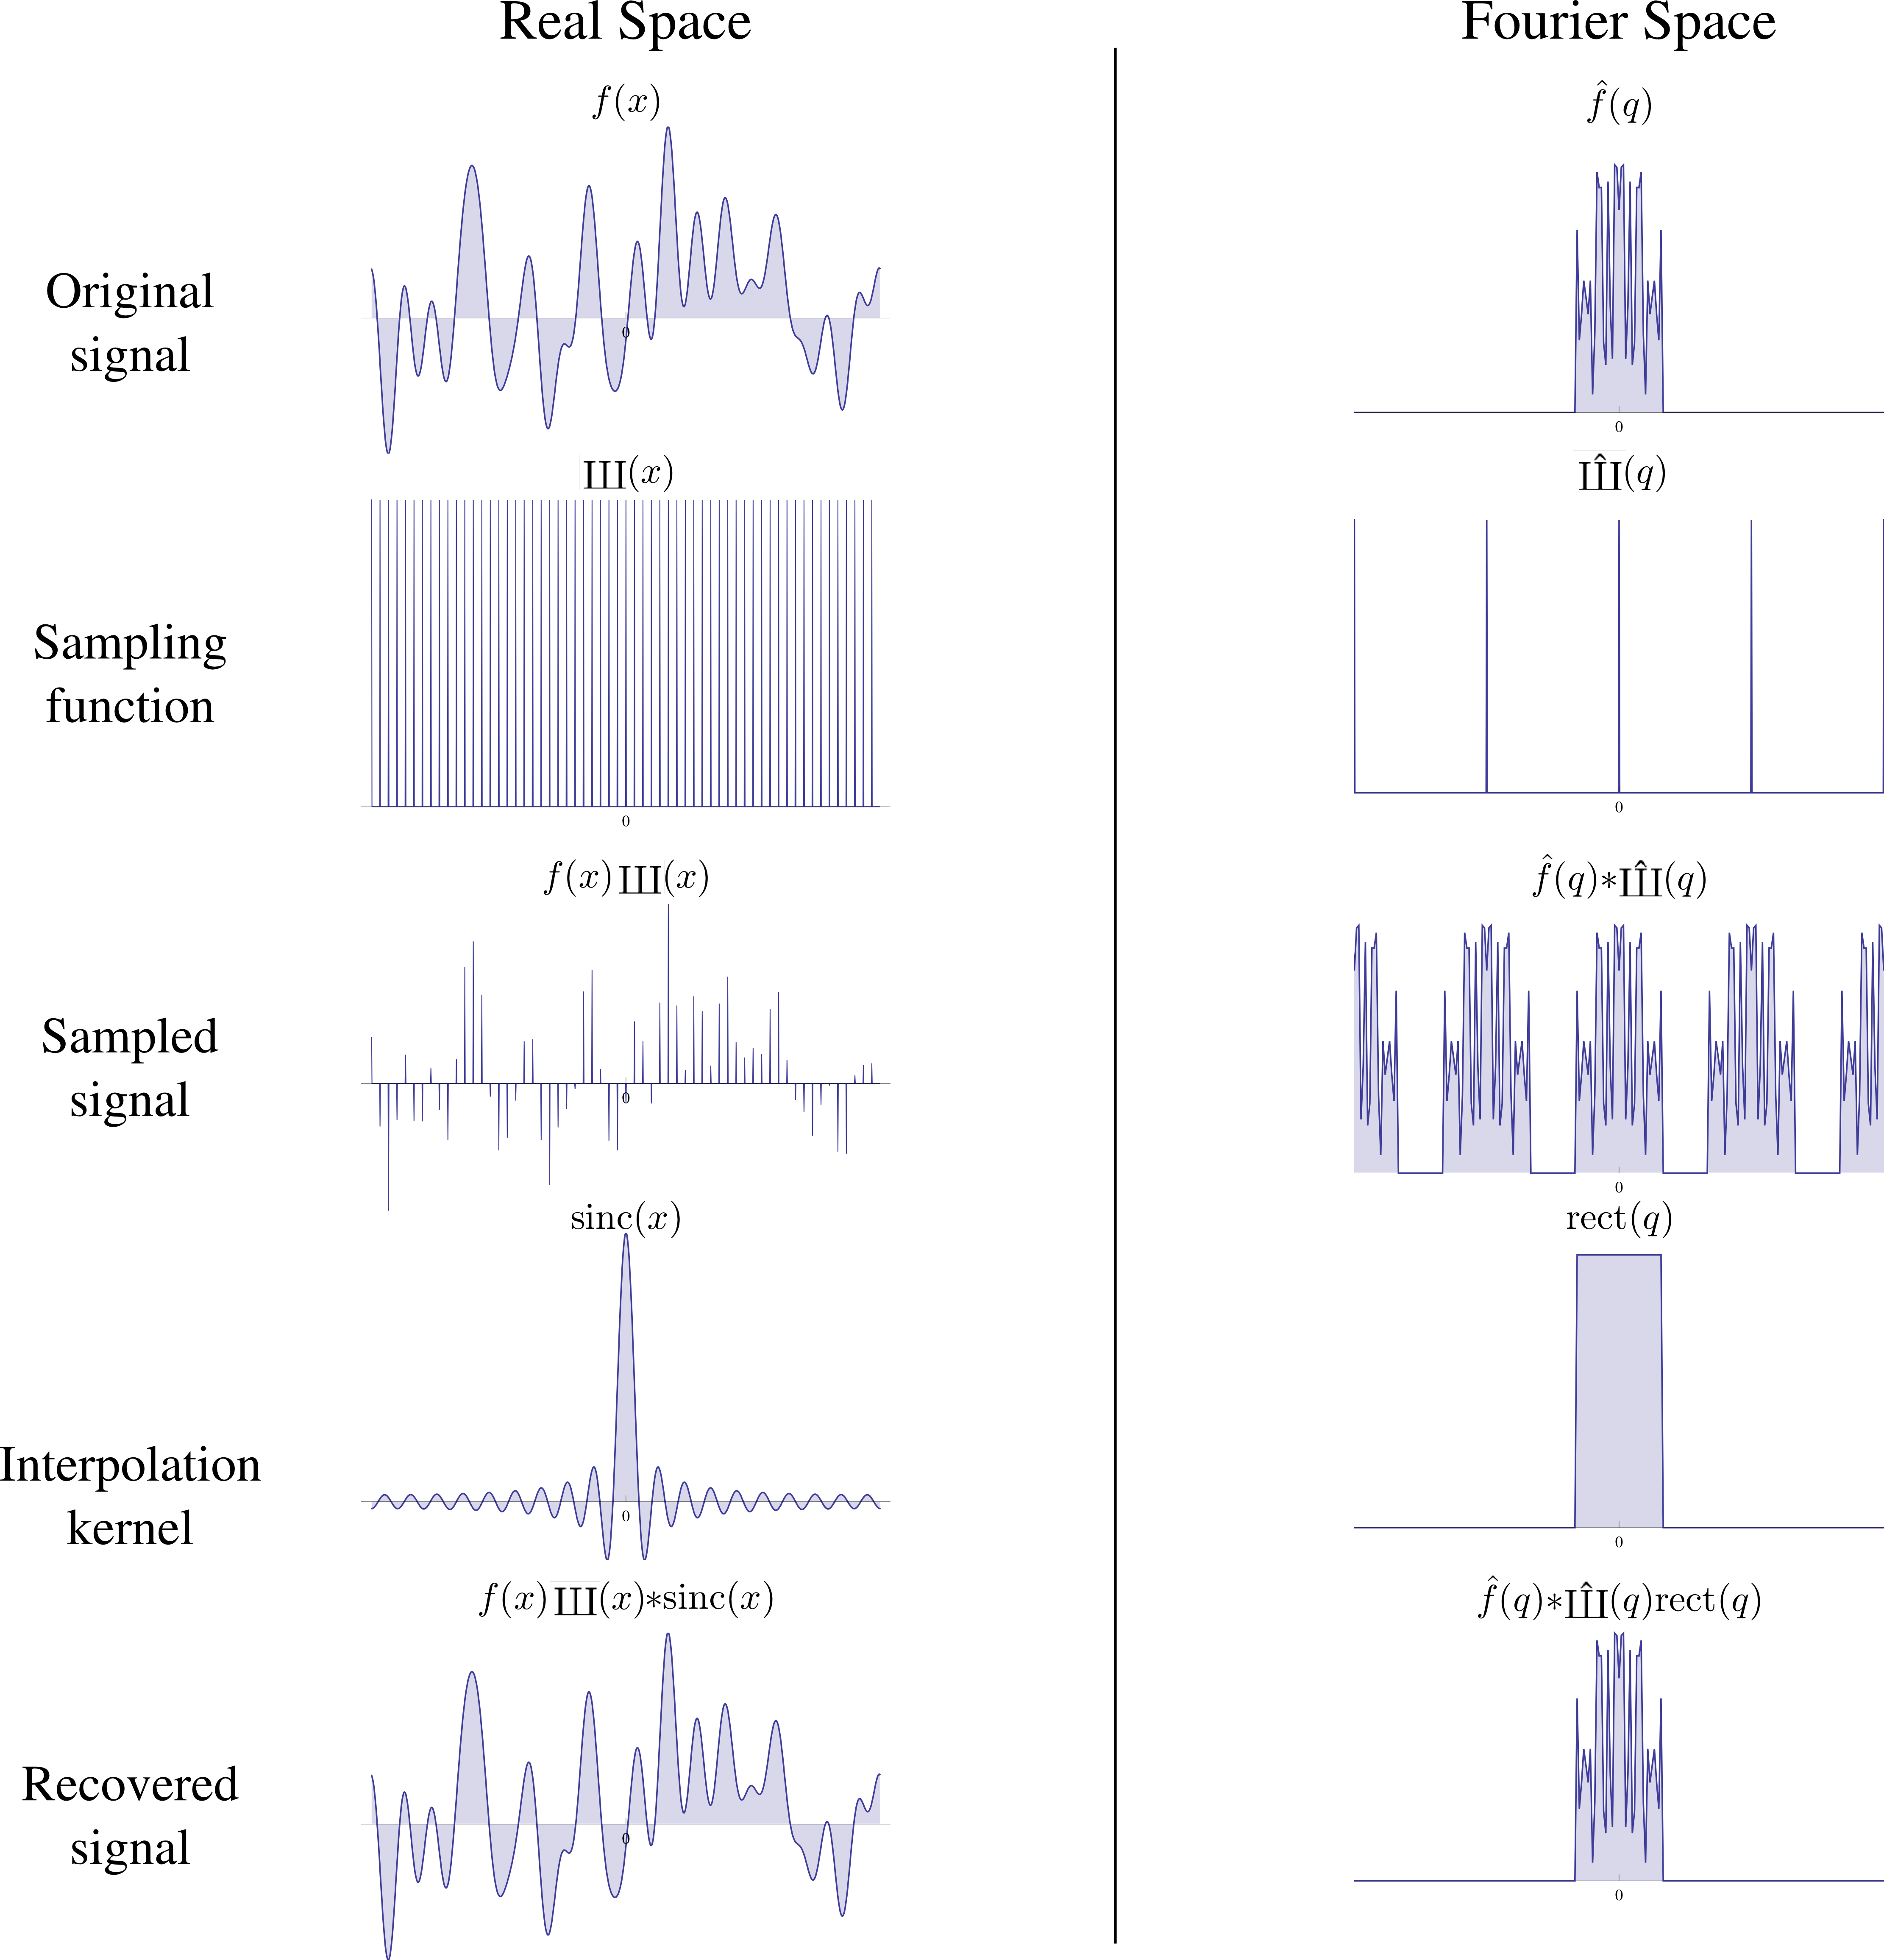
\includegraphics[width=0.9 \columnwidth]{Fourier_Theory/Sampling2.png}
  \caption{Reconstruction of a band-limited signal from discrete samples taken at
    a frequency higher than the Nyquist rate. The signal $f(x)$ is multiplied
    with the sampling function \Sha$(x)$ corresponding to sampling of the signal
    by a pixel detector. This corresponds to replicating the spectrum of the
    signal in Fourier space. Notice that there is no overlap of the replicated
    spectra. It is then possible to recover the original signal by selecting the
    original signal with an appropriate rectangular window function
    rect$(q)$. In real space this corresponds to a convolution with the
    corresponding sinc function sinc$(x)$.}
  \label{Fig:Sampling}
\end{figure}

As figure \ref{Fig:Sampling} shows sampling a signal causes its spectrum to be
replicated in Fourier space. The distance between the replicas is proportional
to the sampling frequency due to the scaling property of the Fourier
transform. If the sampling frequency is below the Nyquist rate the spectra will
overlap and a perfect reconstruct is no longer possible, a phenomenon known as
aliasing (see Fig. \ref{Fig:Undersampling}). We call such a signal {\em undersampled}. If on the other hand
the sampling frequency is higher than the Nyquist rate, we call it {\em
  oversampled} and we define the {\em oversampling ratio}, $\sigma$, as the ratio between the
sampling frequency and the Nyquist rate, or equivalently the fraction between
the center of two replicas of the spectrum in Fourier space and the region for
which the spectrum is different from zero, as illustrated in figure \ref{Fig:OversamplingRatio}.

\begin{figure}[h!]
  \centering
  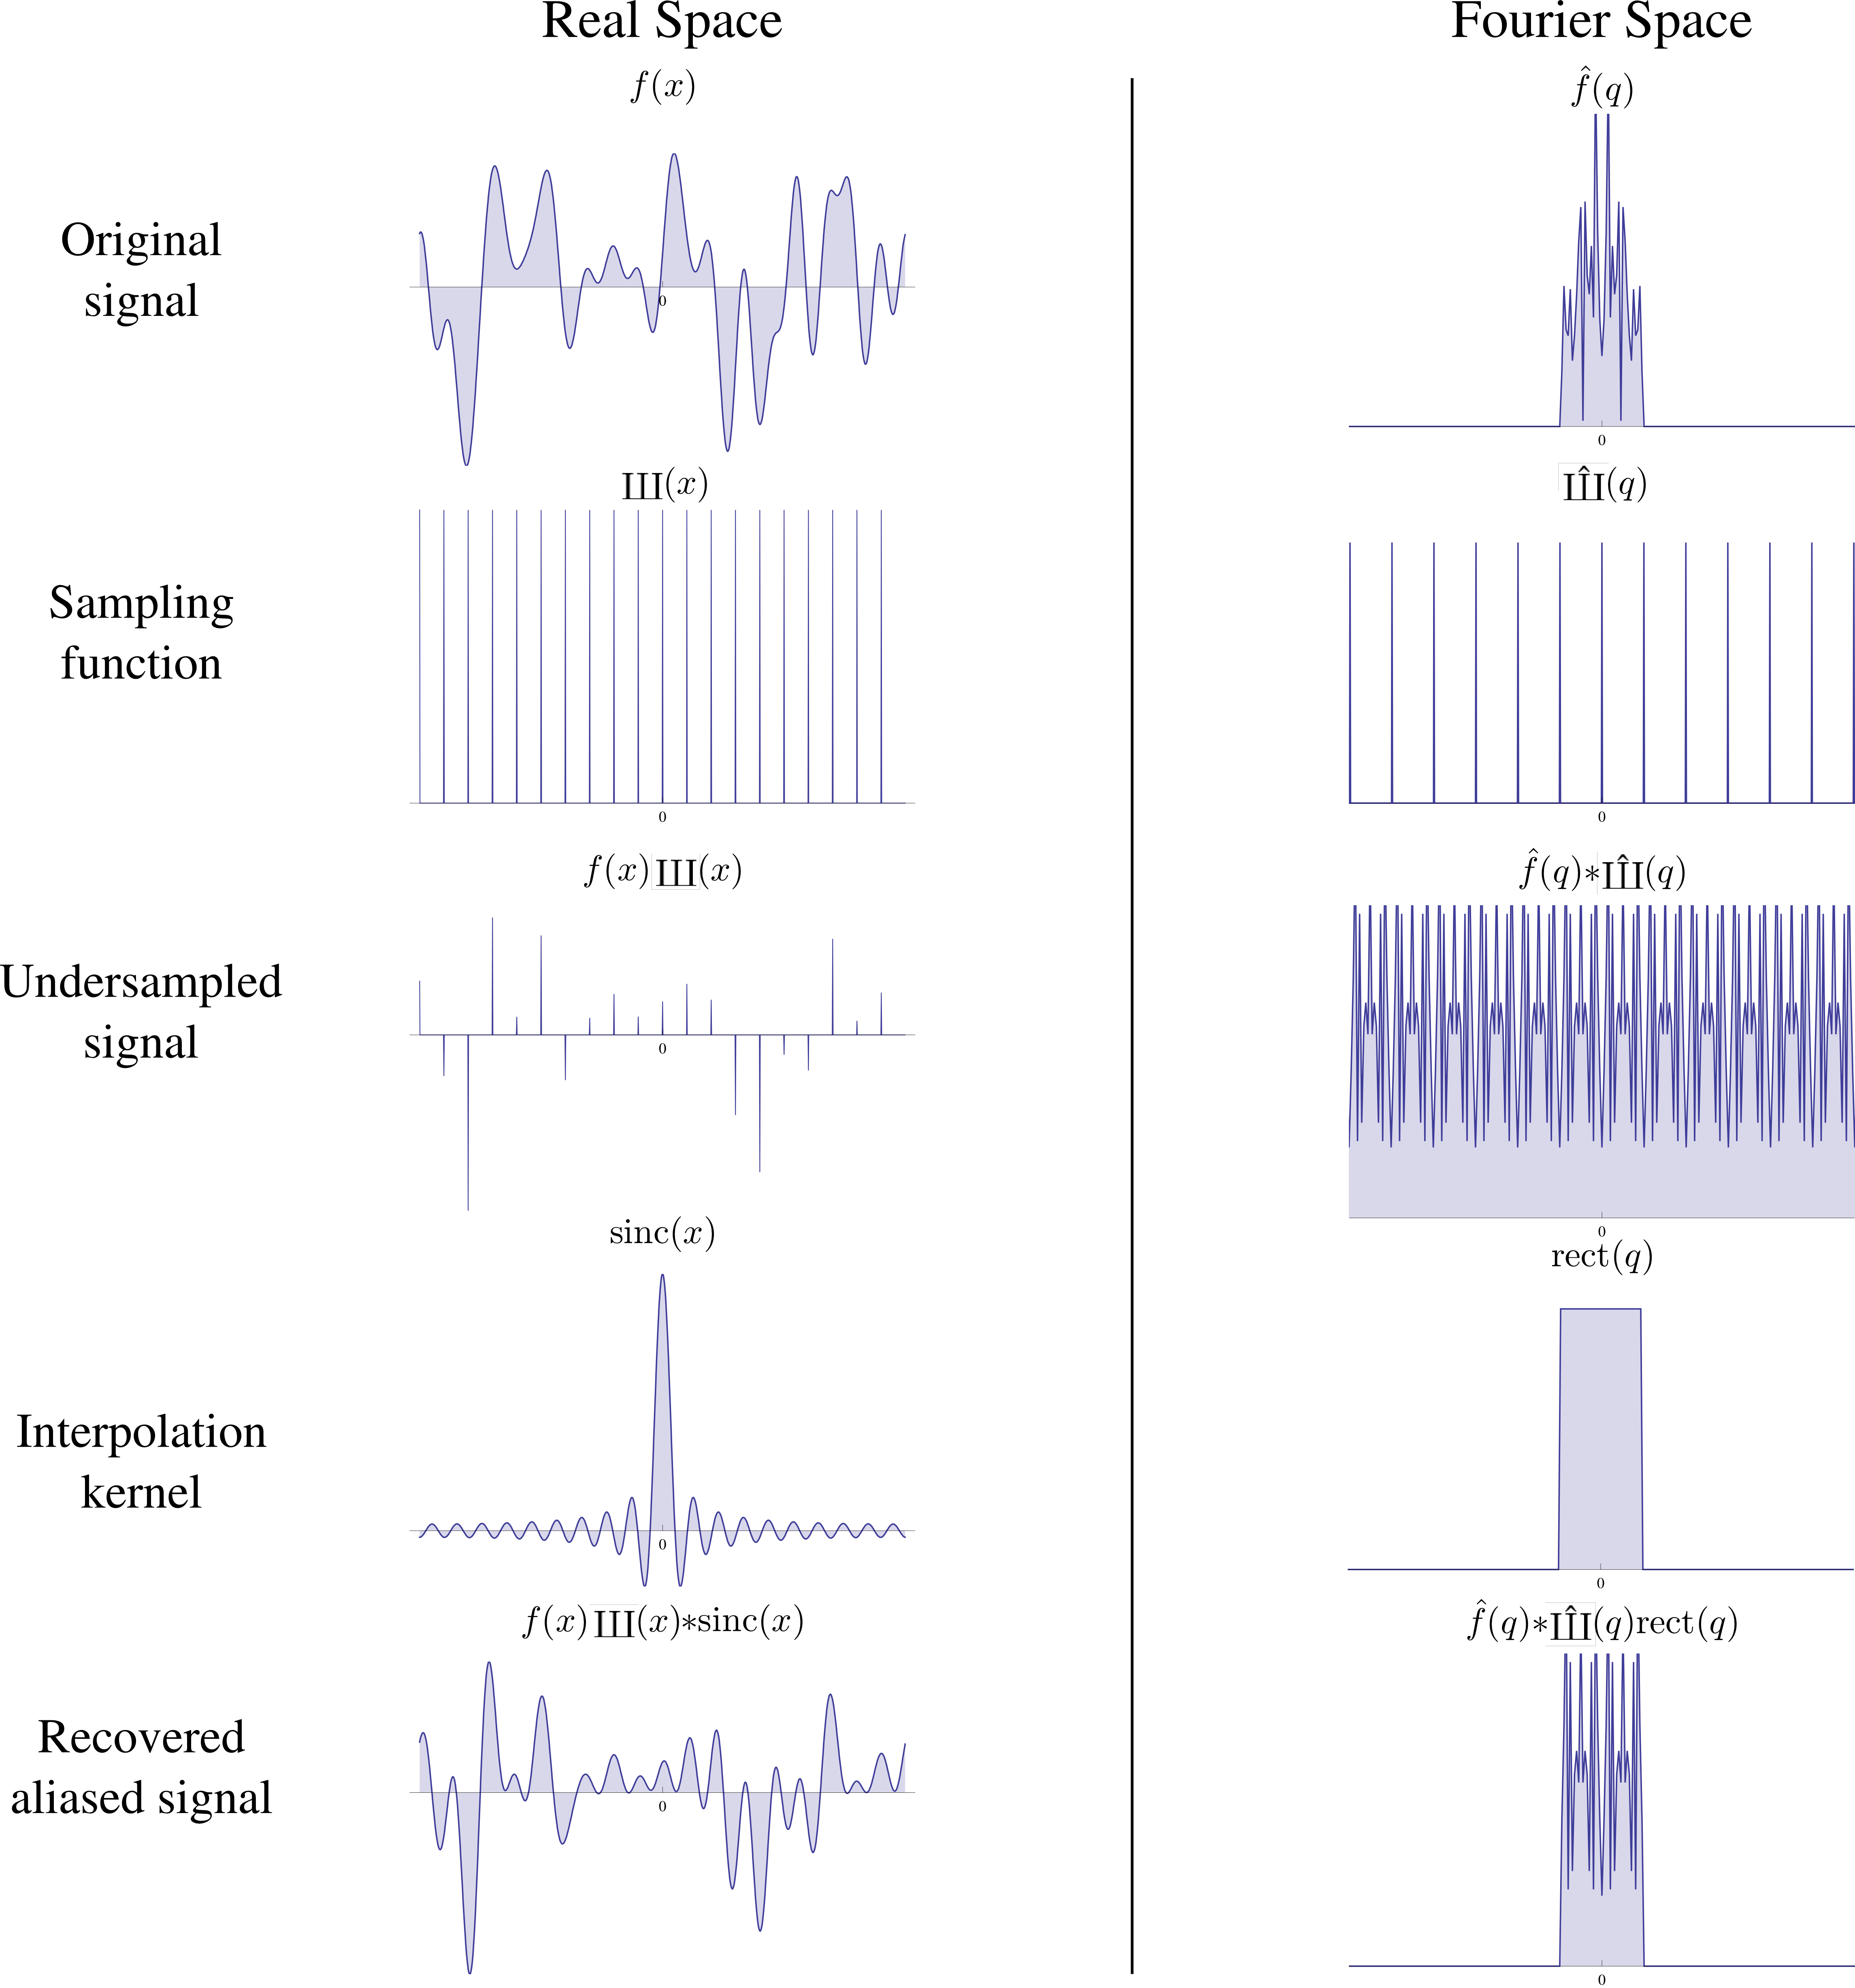
\includegraphics[width=0.9 \columnwidth]{Fourier_Theory/Sampling3.png}
  \caption{Recovery of an undersampled band-limited signal leading to
    aliasing. The process is analogous to \ref{Fig:Sampling} but with a sampling
    frequency below the Nyquist rate. The spectrum of the signal will then
    overlap in the sampled signal and a perfect reconstruction is no longer possible.}
  \label{Fig:Undersampling}
\end{figure}

\begin{figure}[h]
  \centering
  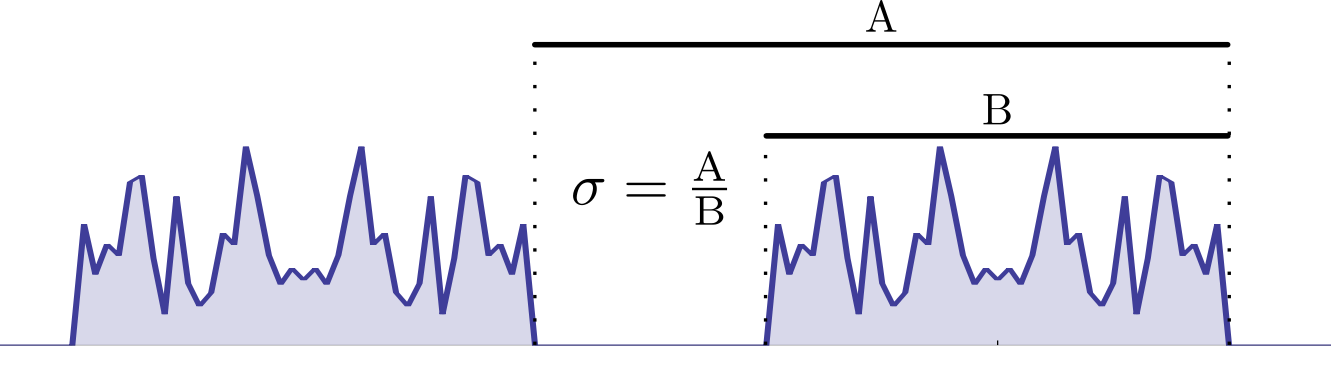
\includegraphics[width=0.8 \columnwidth]{Fourier_Theory/Oversampling.png}
 \caption{The oversampling ratio, denoted by $\sigma$, is the ratio between the
    size of the Fourier space and the region used by the signal.}
  \label{Fig:OversamplingRatio}

\end{figure}
%%% Local Variables: 
%%% mode: latex
%%% TeX-master: "../Thesis"
%%% End: 

\chapter{Theory of X-ray Diffraction by Matter}\label{diffraction_theory}\noindent

This chapter gives an overview of the most important tools necessary to
understand X-ray diffraction and provides a simple framework for analysing most
CXDI experiments based on the first-order Born approximation, also known as
"kinematical" or "single-scattering" approximation. This will be of fundamental
importance when we later try to reconstruct the object that gave rise to a given
diffraction pattern, as  it is obviously impossible to do this if we cannot
predict the diffraction pattern that a given object produces.

\section{Scattering by a free electron}\label{diffraction_physics}

According to classical electromagnetic theory when a plane monochromatic wave of
amplitude $E_0$, frequency $\nu$, propagating along the $z$ axis
(Fig. \ref{coordinate_axis}a), given by
\begin{equation}
E_i(z,t) = E_0 \exp(2 \pi i \nu (t-z/c)) \, ,
\label{Eq:wave_propagation}
\end{equation}
travels through an electron of charge $e$ and mass $m$ located at the origin of a coordinate
system, that electron will oscilate in the direction of the incident electric 
vector driven by
\begin{equation}
a(t) = \frac{e E_i(0,t)}{m}
\label{Eq:electron_acceleration}
\end{equation}
with a frequency equal to the incoming wave. This in turn will make it radiate
an electric field $E_s$, like any accelerating charge. It follows from Maxwell's
equations that the electric field generated by an accelerating electron is given by
\begin{equation}
E_s( \mathbf r,t) = \frac{e a_{\perp}(t - |\mathbf r|/c)}{4 \pi \epsilon_0 c^2 r}
\label{Eq:scattering_by_accelerating_charge}
\end{equation}
where  $\epsilon_0$ is the permittivity of free space and $a_{\perp}$ is the acceleration projected on a plane normal to $r$, also called the transverse component of the acceleration (Fig. \ref{coordinate_axis}b). 
\begin{figure}[h]
\centering
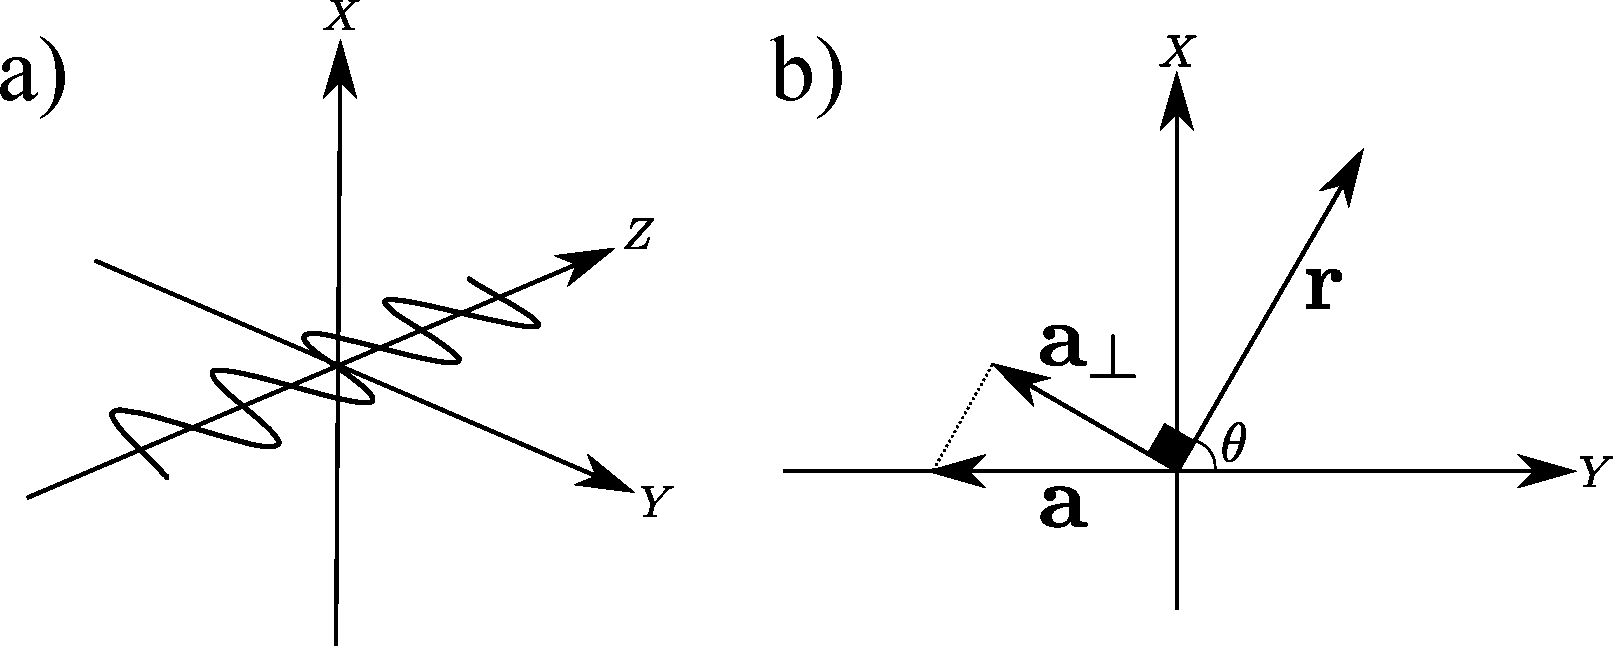
\includegraphics[width=1 \columnwidth]{Diffraction_Theory/coordinate_acceleration.pdf}
\caption{{\bf a)} Monochromatic planar wave linearly polarized along the $y$ axis
  propagating in the positive $z$ direction. {\bf b)} Transverse component of the
  acceleration sustained by the electron as observed from the position ${\mathbf r}$. $\theta$ is the angle between the polarization axis and the projection of $\mathbf r$ on a plane normal to the propagation direction.}
\label{coordinate_axis}
\end{figure}
Finally combining equations \ref{Eq:wave_propagation},\ref{Eq:electron_acceleration} and \ref{Eq:scattering_by_accelerating_charge} we get that the instantaneous scattered field by a free electron is given by
\begin{eqnarray}
a_{\perp}(t) & = & |\mathbf a(t)| \sin \theta  \\
E_s(\mathbf r,t) & = & \frac{e^2 E_0 \sin \theta }{4 \pi \epsilon_0 m c^2 r} \exp(2 \pi i \nu (t -| \mathbf r|/c)) 
\label{Eq:scattering_by_electron}
\end{eqnarray}
The classical electron radius is defined as,
\begin{equation}
r_e = \frac{e^2}{4 \pi \epsilon_0 m c^2}
\end{equation}
which can be used to simplify the electric field expression to,
\begin{equation}
E_s(\mathbf r,t) = \frac{r_e E_0 \sin \theta }{r} \exp(2 \pi i \nu (t -| \mathbf
r|/c))  \, .
\label{Eq:scattering_by_electron_simplified}
\end{equation}
The time averaged scattered power per unit area normal to $\mathbf r$, also
known as intensity, can then be obtained from the average length of the Poynting vector,
\begin{equation} 
I(\mathbf r) = \frac{ |E_{max}(\mathbf r)|^2 }{2 \epsilon_0 c} .
\label{Eq:poynting_vector}
\end{equation}
where $E_{max}$ denotes the maximum value of the electric field.
The time averaged power per unit area normal to $\mathbf r$ scattered by an electron is then,
\begin{equation}
I(\mathbf r)  = \frac{r_e^2 E_0^2 \sin^2 \theta }{2 \epsilon_0 c r^2} \, ,
\label{Eq:scattered_intensity}
\end{equation}
The total scattered intensity by a free electron as a fraction of the incoming
intensity, can now be calculated by integrating equation
\ref{Eq:scattered_intensity} over a spherical shell of radius 1 around the electron,
\begin{eqnarray}
I_0 & = & \frac{E_0^2}{2 \epsilon_0 c} \\
I_s & = & \int\limits_0^{2 \pi} \int\limits_0^{\pi} \frac{r_e^2 E_0^2 \sin^2
  \theta }{2 \epsilon_0 c} \sin \theta d \theta d\phi = \frac{8 \pi}{3}
\frac{r_e^2 E_0^2}{2 \epsilon_0 c} \\
\sigma_T & = & \frac{I_s}{I_0} = \frac{8 \pi}{3} r_e^2
\end{eqnarray}
where $I_0$ represent the incoming intensity, $I_s$ the scattered intensity and
$\sigma_T$ the ratio between the two, also known as the {\em scattering cross-section}
for a free electron, also known as the Thomson cross-section after the British
physicist J.J. Thomson who first derived it in the beggining of the 20th
century. Elastic scattering by a free charged particle is also known as {\em Thomson scattering}.

\section{Scattering by two electrons}\label{diffraction_physics}

If instead of just one electron we have a system composed of two or more
electrons a new phenomenon is observed, {\em interference} between the waves
scattered by the different electrons. We'll start by looking at the most simple
system where this occurs, one with just two electrons. We'll keep the electron
from the previous section at the origin and add a new electron at the position
$\mathbf r$. When the system is illuminated by an electric field of amplitude $E_0$
traveling along $\mathbf s_0$ both electrons will scatter as described in
Eq. \ref{Eq:scattering_by_electron_simplified}. The amplitude of the scattered
field from each electron is the same but the phase depends on the position of
the electron (Fig. \ref{Fig:two_electrons}). 

\begin{figure}[h]
\begin{center}
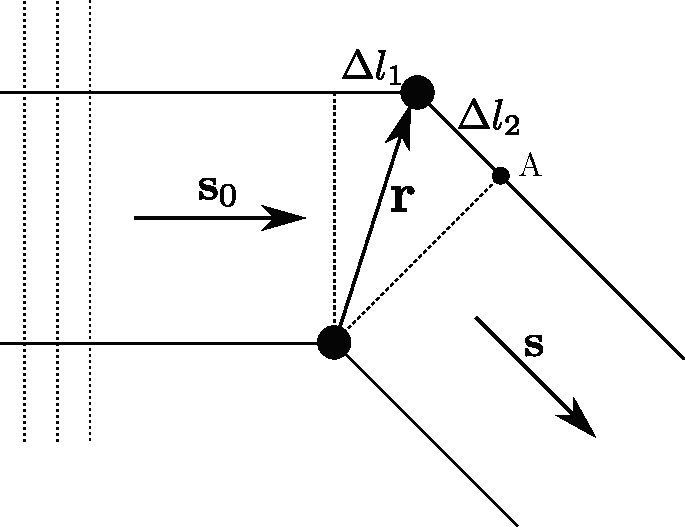
\includegraphics[width=0.7 \columnwidth]{Diffraction_Theory/two_electrons.pdf}
\end{center}
\caption{Monochromatic planar propagating along $\mathbf s_0$ shines on two
  electrons separated by $\mathbf r$. The observed scattered electric field on the
  direction $\mathbf s$ at a distance $| \mathbf d|$ much larger than $|\mathbf r|$ is the
  sum of two identical fields separated by a phase difference dependent on the path difference $\Delta l_1 + \Delta l_2$.}
\label{Fig:two_electrons}
\end{figure}
For an observer located at $\mathbf d$ in the direction of $\mathbf s$, at a distance
much greater than the distance between the electrons the observed total electric
field is the sum of the fields scattered by each of the electrons, which can be
approximated by,
\begin{eqnarray}
\Delta l & = & \Delta l_1 + \Delta l_2 = \mathbf r \cdot (\mathbf s_0 - \mathbf s)\\
E(\mathbf d) & = & E_s(\mathbf d) + E_s(\mathbf d) \exp(\frac{2 \pi i \Delta l}{\lambda})
\end{eqnarray}
where $\mathbf s_0$ and $\mathbf s$ are unit vectors, $\Delta l$ the total path
difference, $E_s$ the electric field scattered by an isolated electron, $\lambda$
the walength of the incoming field and $E$ the total observed field.
This approximation assumes that the $|\mathbf d| -
|\mathbf d- \mathbf a| << \lambda$ or put in another way $|\mathbf r|^2/(|\mathbf d| \lambda) \ll
1 $. This approximation is known as the {\em Fraunhofer approximation} and the conditions
under which they are valid are known as the far field regime. Fraunhoffer
diffraction is also used to describe diffraction in this regime. Also implicit
in this calculation is the assumption that the scattered field from one electron produces a
negligible scattered field on the other electron, that is, multiple
scattering can be ignored. This approximation is known as the {\em first-order Born
  approximation}.
It is
important to notice that the relative phase between the two electrons does not
depend on the choice of origin and so the observed intensity is independent of
the choice of origin, as it must obviously be. 


\section{Scattering by an arbitrary electron cloud}\label{diffraction_physics}

The two electron framework presented in the previous section can be easily
extended to $N$ electrons by noticing that the electrons scatter independently
of each other. So the scattering of $N$ electrons measured at a point $\mathbf d$
is given by,
\begin{equation}
E(\mathbf d) = E_s(\mathbf d) \sum_{n=0}^N \exp\left(\frac{2 \pi i \mathbf r_n \cdot(\mathbf s_0 -
\mathbf s)}{\lambda}\right) \, .
\end{equation}
The vector $\mathbf S = \frac{\mathbf s_0 - \mathbf s}{\lambda}$ is known in crystallography
as the {\em scattering vector} and the surface drawn by the tip of the
scattering vector while $\mathbf s$ is rotated around a sphere is known as the
{\em Ewald sphere}.

The continuous case is now easily derived by replacing individual electrons by
an electron density $\rho$. The scattering from an electron density cloud is
then described by,
\begin{equation}
E(\mathbf d) = E_s(\mathbf d) \int_{\mathbf r} \rho(\mathbf r) \exp\left(2
    \pi i \mathbf r \cdot \mathbf S \right) d\mathbf r\, .
\end{equation}
We can now introduce the {\em structure factor}, defined as the ratio between
the scattered field by the system and the scattered field by a single
electron,
\begin{equation}
F(\mathbf d) = \frac{E(\mathbf d)}{E_s(\mathbf d)} = F\left(\frac{\mathbf d}{|\mathbf d|}\right)
\end{equation}
The structure factor is a more useful quantity than the electric field as it does not depend
on the distance to the detector, only on the direction of the observer and the
structure of the system. For an arbitrary electron cloud the structure factor as
a function of the scattering vector is given by,
\begin{equation}
F(\mathbf S) = \int_{\mathbf r} \rho(\mathbf r) \exp\left(2
    \pi i \mathbf r \cdot \mathbf S \right) d\mathbf r\, ,
\end{equation}
which is simply the three dimensional Fourier transform of $\rho(\mathbf r)$
evaluated at $\mathbf S$. It is for this reason that Fourier transforms are such
a useful tool when studying diffraction, and why they were introduced in the
previous chapter.


{\em ADD SOMETHING ABOUT COHERENCE AND INCOHERENCE}
%%% Local Variables: 
%%% mode: latex
%%% TeX-master: "../Thesis"
%%% End: 

\chapter{Image Reconstruction}\label{Image Reconstruction}\noindent

In the previous chapter we have developed tools that allow us to predict
and calculate the X-ray diffraction pattern from an arbitrary electron density,
using mild assumptions. In this chapter we will try to tackle the {\em inverse
  problem}, that is, from an arbitrary diffraction pattern we will try to
recover the electron density that gave rise to it.
\section{The Phase Problem}

We have seen that a diffraction pattern can be calculated from the Fourier
transform of the electron density. We have also seen in chapter
\ref{fourier_transform_basics} that the inverse of the Fourier transform is
exactly like the Fourier transform, except with the sign of the exponent
swapped. So we should be able to recover the electron density by,
\begin{equation}
\rho(\mathbf r) = \int_{\mathbf r} F(\mathbf S) \exp\left(-2
    \pi i \mathbf r \cdot \mathbf S \right) d\mathbf S\, .
\end{equation}

In general $F(\mathbf S)$ is a complex number and unfortunately it is not
possible to measure $F(\mathbf S)$, but only its absolute value, also known as
amplitude. The phase, also known as the argument of $F(\mathbf S)$, is not known and so
this problem is often called the {\em phase problem}. One could try to reconstruct the
object assuming that the phases have an arbitrary value, say 0, and use the
experimental intensities but this usually gives an uninterpretable picture. On
the other hand if the phases were known and the amplitudes unknown, then the
resulting picture is still quite similar to the original, suggesting that the
phases carry more structural information than the amplitudes (see Fig. \ref{Fig:PhaseSwapping}).
\begin{figure}[h]
  \centering
  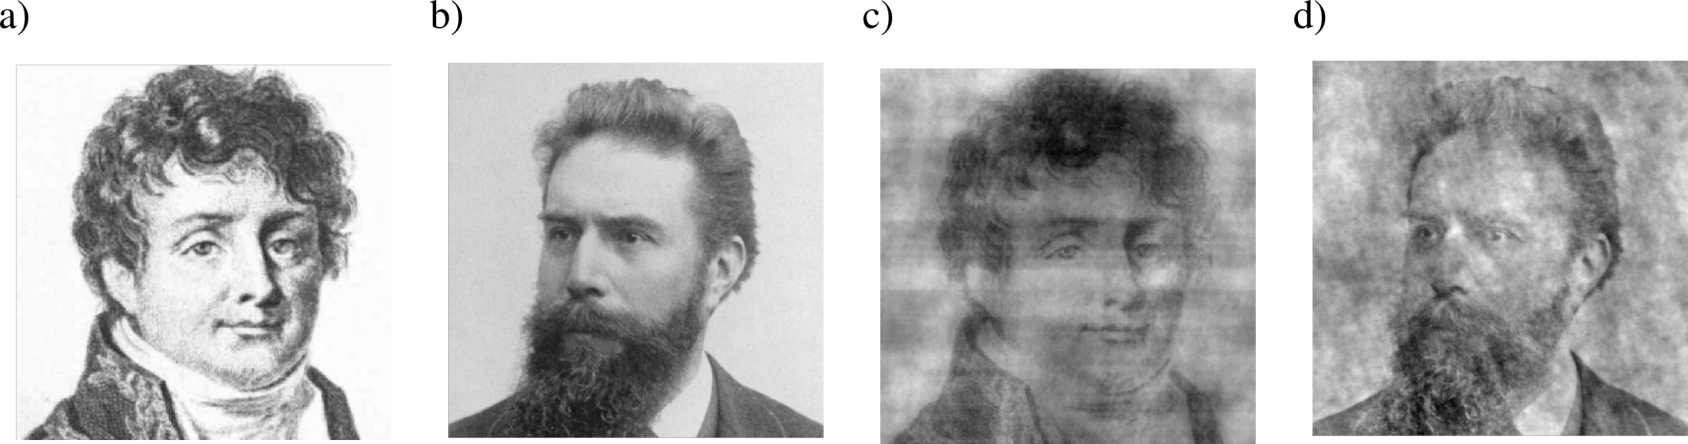
\includegraphics[width=1 \columnwidth]{Image_Reconstruction/PhaseSwapping2.png}
  \caption{Portraits of Jean-Baptiste Fourier (a) and Wilhelm R\"{o}ntgen (b).
    {\bf c)} Fourier synthesis using the amplitudes from b and the phases from
    a. {\bf d)}
    Fourier synthesis using the amplitudes from a and the phases from b.}
  \label{Fig:PhaseSwapping}
\end{figure}

If nothing about the object being imaged is known then the problem is
undetermined, as for a pattern with $N$ pixels we have $2N$ unknowns (the real and
imaginary part of the object) but only $N$ constraints. But if we known that the object is isolated, meaning the
object is surrounded by a constant $\rho$ (e.g., sample in vacuum where
surrounding $\rho = 0$), then in some circumstances it is possible to solve this
problem. The number of pixels of the object must at least be half of that of the
diffraction pattern for the number of unknowns match the number of
constraints, that is the oversampling ratio (see Fig. \ref{Fig:OversamplingRatio}) of the image must be bigger than
two, or equivalently the object must occupy less than half of the field of
view. We will call images which fulfill this condition {\em oversampled}.

But this is not enough being able to solve the problem. In fact it
has long been known that the problem is often undetermined in one dimension
\cite{Walther63}. Fortunately for higher dimensions is has been proven it has
been proven that most oversampled patterns have unique solutions
\cite{Bruck79}. This difference derives from the fact that one-dimensional
polynomials are factorizable unlike two or higher dimension ones.

\section{Image Reconstruction Algorithms}

Knowing that the two or higher dimensional phasing problem for oversampled
patterns has a unique solution in most cases is a necessary starting point to
solve the phase problem, but a method to find that unique solution is still
necessary. The phase problem is remarkably difficult since it is neither a
linear nor a convex problem. That makes it a nonconvex problem in a very high
dimensional space, which is a class of problems that is very challenging.

\begin{figure}[h]
  \centering
  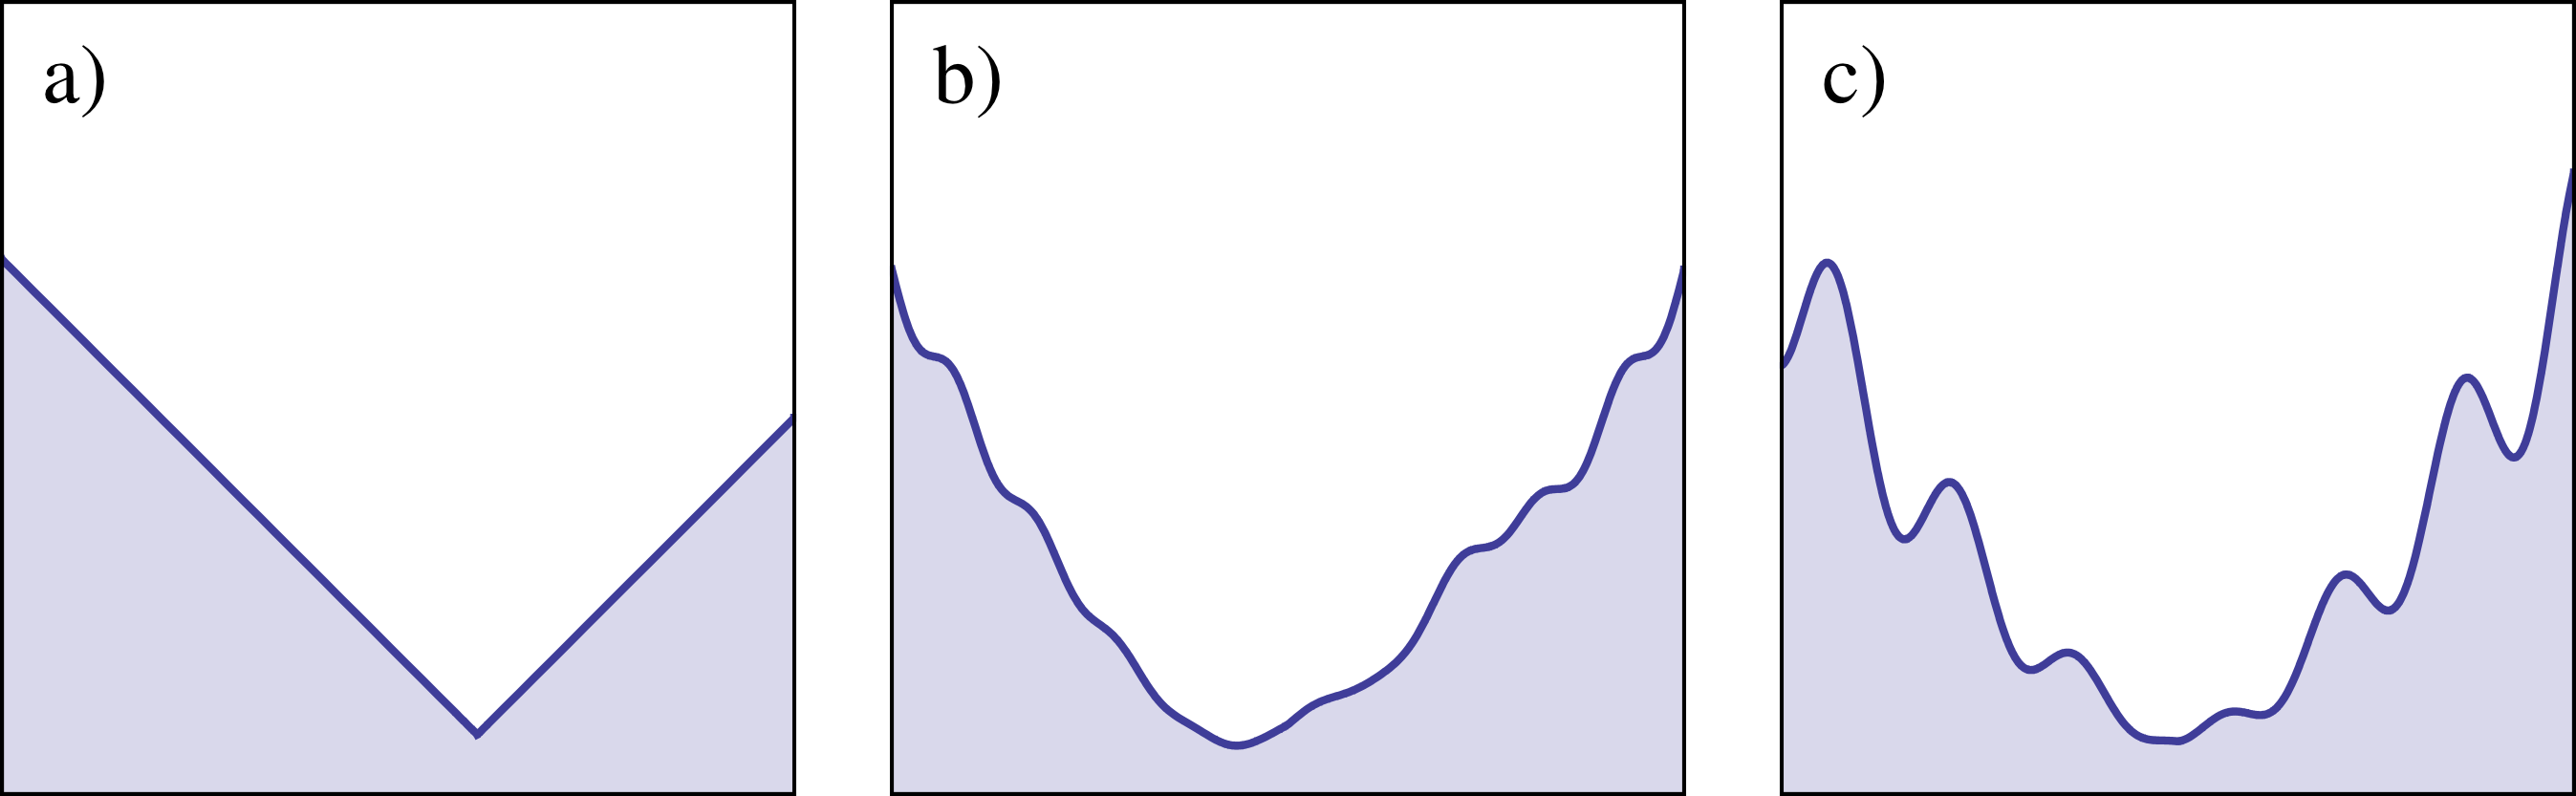
\includegraphics[width=1 \columnwidth]{Image_Reconstruction/convexity.png}
  \caption{Function to be minimized for a linear (a), convex (b) and nonconvex
    (c) optimization problems.}
  \label{Fig:Convexity}
\end{figure}

In 1972 Gerchberg and Saxton \cite{Gerchberg72} introduced an iterative algorithm to solve
a related problem, that of obtaining phase information using both the
diffraction pattern and an electron micrograph of a sample. The iteration starts
by Fourier transforming the real space input, $\rho_i(\mathbf x)$. Then it
replaces the resulting amplitudes with the square root of the intensities,
$I(\mathbf S)$. The result is then back Fourier transformed and the amplitudes
of the resulting images are replaced by the ones from the electron micrograph $M(\mathbf r)$.
\begin{algorithm}
\caption{Gerchberg-Saxton Iteration}
\begin{algorithmic}
  \STATE $F_{i}(\mathbf S) \gets \mathscr{F}\{\rho_i(\mathbf r)\}$
  \STATE $F_{i+1}(\mathbf S) \gets \sqrt{I(\mathbf S)} \frac{F_i(\mathbf S)}{|F_i(\mathbf S)|}$
  \STATE $\rho_{i+1}(\mathbf r) \gets M(\mathbf r)
  \frac{\mathscr{F}^{-1}\{F_{i+1}(\mathbf
    S)\}}{|\mathscr{F}^{-1}\{F_{i+1}(\mathbf S)\}|}$
\end{algorithmic}
\end{algorithm}

In 1978 Fienup \cite{Fienup78}, inspired by the above algorithm, introduced the error
reduction algorithm to solve the phasing problem. Instead of using the electron
micrograph as constraints in real space Fienup introduces the concept of {\em
  support} function, $\Pi(\mathbf r)$, which is equal to 1 where the
object is allowed the reside and 0 otherwise. 
The iteration is analogue to the Gerchberg-Saxton but the last step is replaced
by setting all points outside the support to 0.
\begin{algorithm}
\caption{Error Reduction Iteration}
\begin{algorithmic}
  \STATE $F_{i}(\mathbf S) \gets \mathscr{F}\{\rho_i(\mathbf r)\}$
  \STATE $F_{i+1}(\mathbf S) \gets \sqrt{I(\mathbf S)} \frac{F_i(\mathbf S)}{|F_i(\mathbf S)|}$
  \STATE $\rho_{i+1}(\mathbf r) \gets \Pi(\mathbf r) \mathscr{F}^{-1}\{F_{i+1}(\mathbf S)\}$
%  \STATE $i = 0$
\end{algorithmic}
\end{algorithm}

By applying this procedure iteratively it is possible to recover the correct
solution. Unfortunately in practise the algorithm easily gets stuck in
local minima and cannot find the global minimum.

\subsection{Iterations as Projections}

In 1984 Levi and Stark realized that the above iterations can be
interpreted as projections in Hilbert space \cite{Levi84}. This provides a
particularly powerful method for trying to understand these algorithms.
Lets call the replacement of the Fourier space amplitudes with the square root of
the intensities the modulus projection, $P_m$, and the replacement of the image
outside of the support with 0 the support projection, $P_s$. If one treats the
real space image as a vector in a high dimensional space, with one dimension per
pixel, then it is easy to see that $P_s$ is the projection into the hyperplane
spanned by the dimensions corresponding to pixels inside the support. The
modulus projection can also be interpreted as a projection in the space of the
pixels of the diffraction pattern, where each pixel contributes two dimensions,
the real part and the imaginary part (see Fig. \ref{Fig:Projections}). 

\begin{figure}[h]
  \centering
  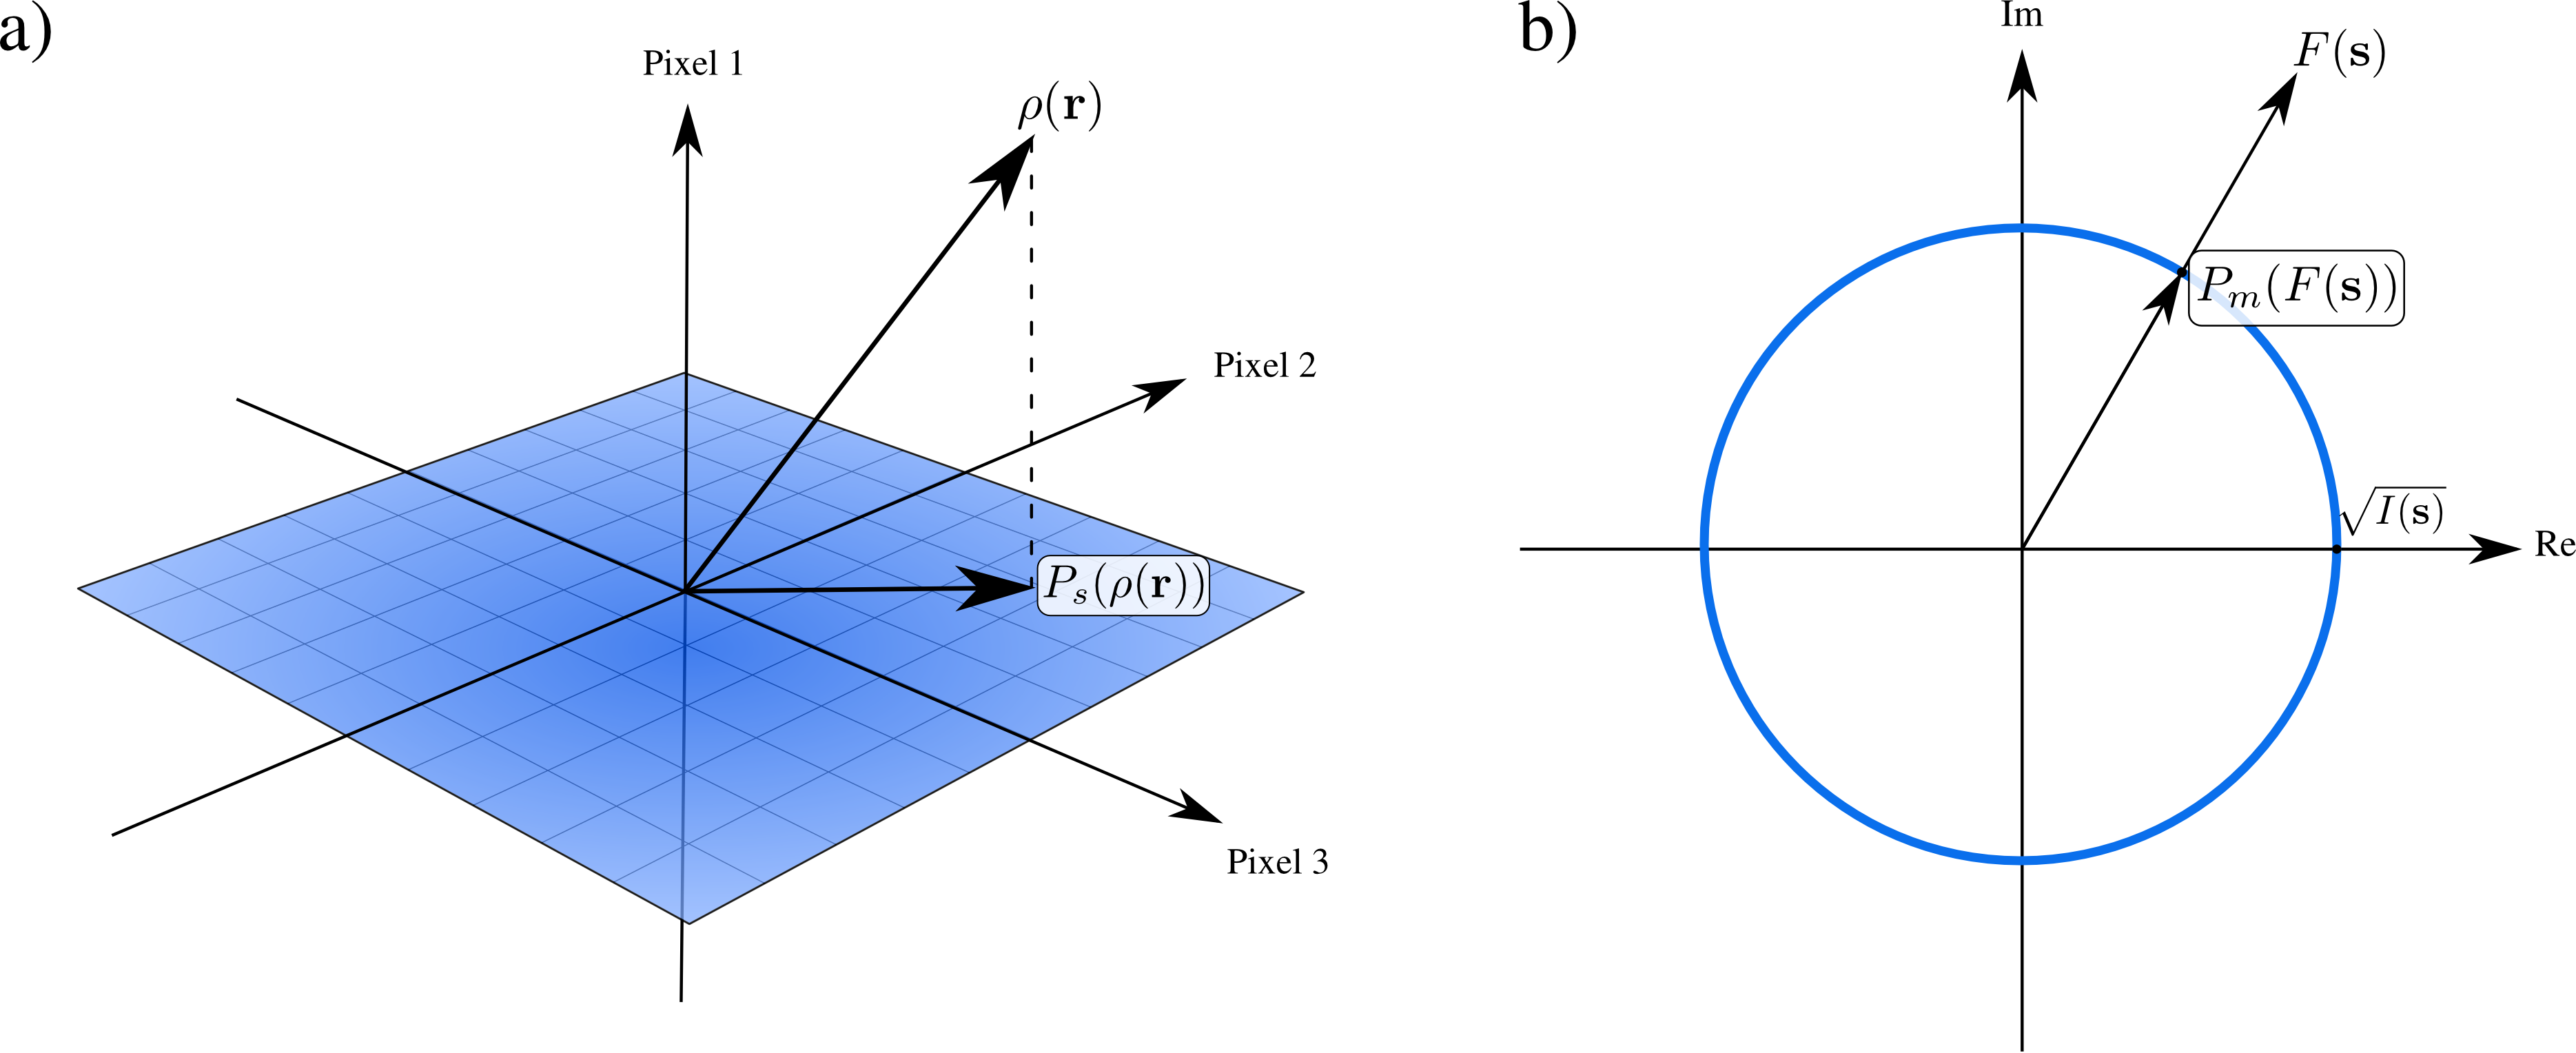
\includegraphics[width=1 \columnwidth]{Image_Reconstruction/projections.png}
  \caption{{\bf a)} Support projection for a 3 pixel image where the support is
    composed of pixels 2 and 3. {\bf b)} Modulus projection for 1 pixel of the
    diffraction pattern.}
  \label{Fig:Projections}
\end{figure}

Due to the distance preserving property of the Fourier transform the modulus
projection is also a projection in real space. The biggest difference between
the two projection is that while the support constraint set is convex, the
modulus constraint is not, not all points between two points of the modulus
constraint set belong to the modulus constraint set.

In this framework of projections the Error Reduction algorithm is simply $P_m$
followed by $P_s$. The fact that it stagnates can then be easily understood in
connection to the non convexity of the modulus constraint as
Fig. \ref{Fig:Stagnation} illustrates.

\begin{figure}[h]
\centering
  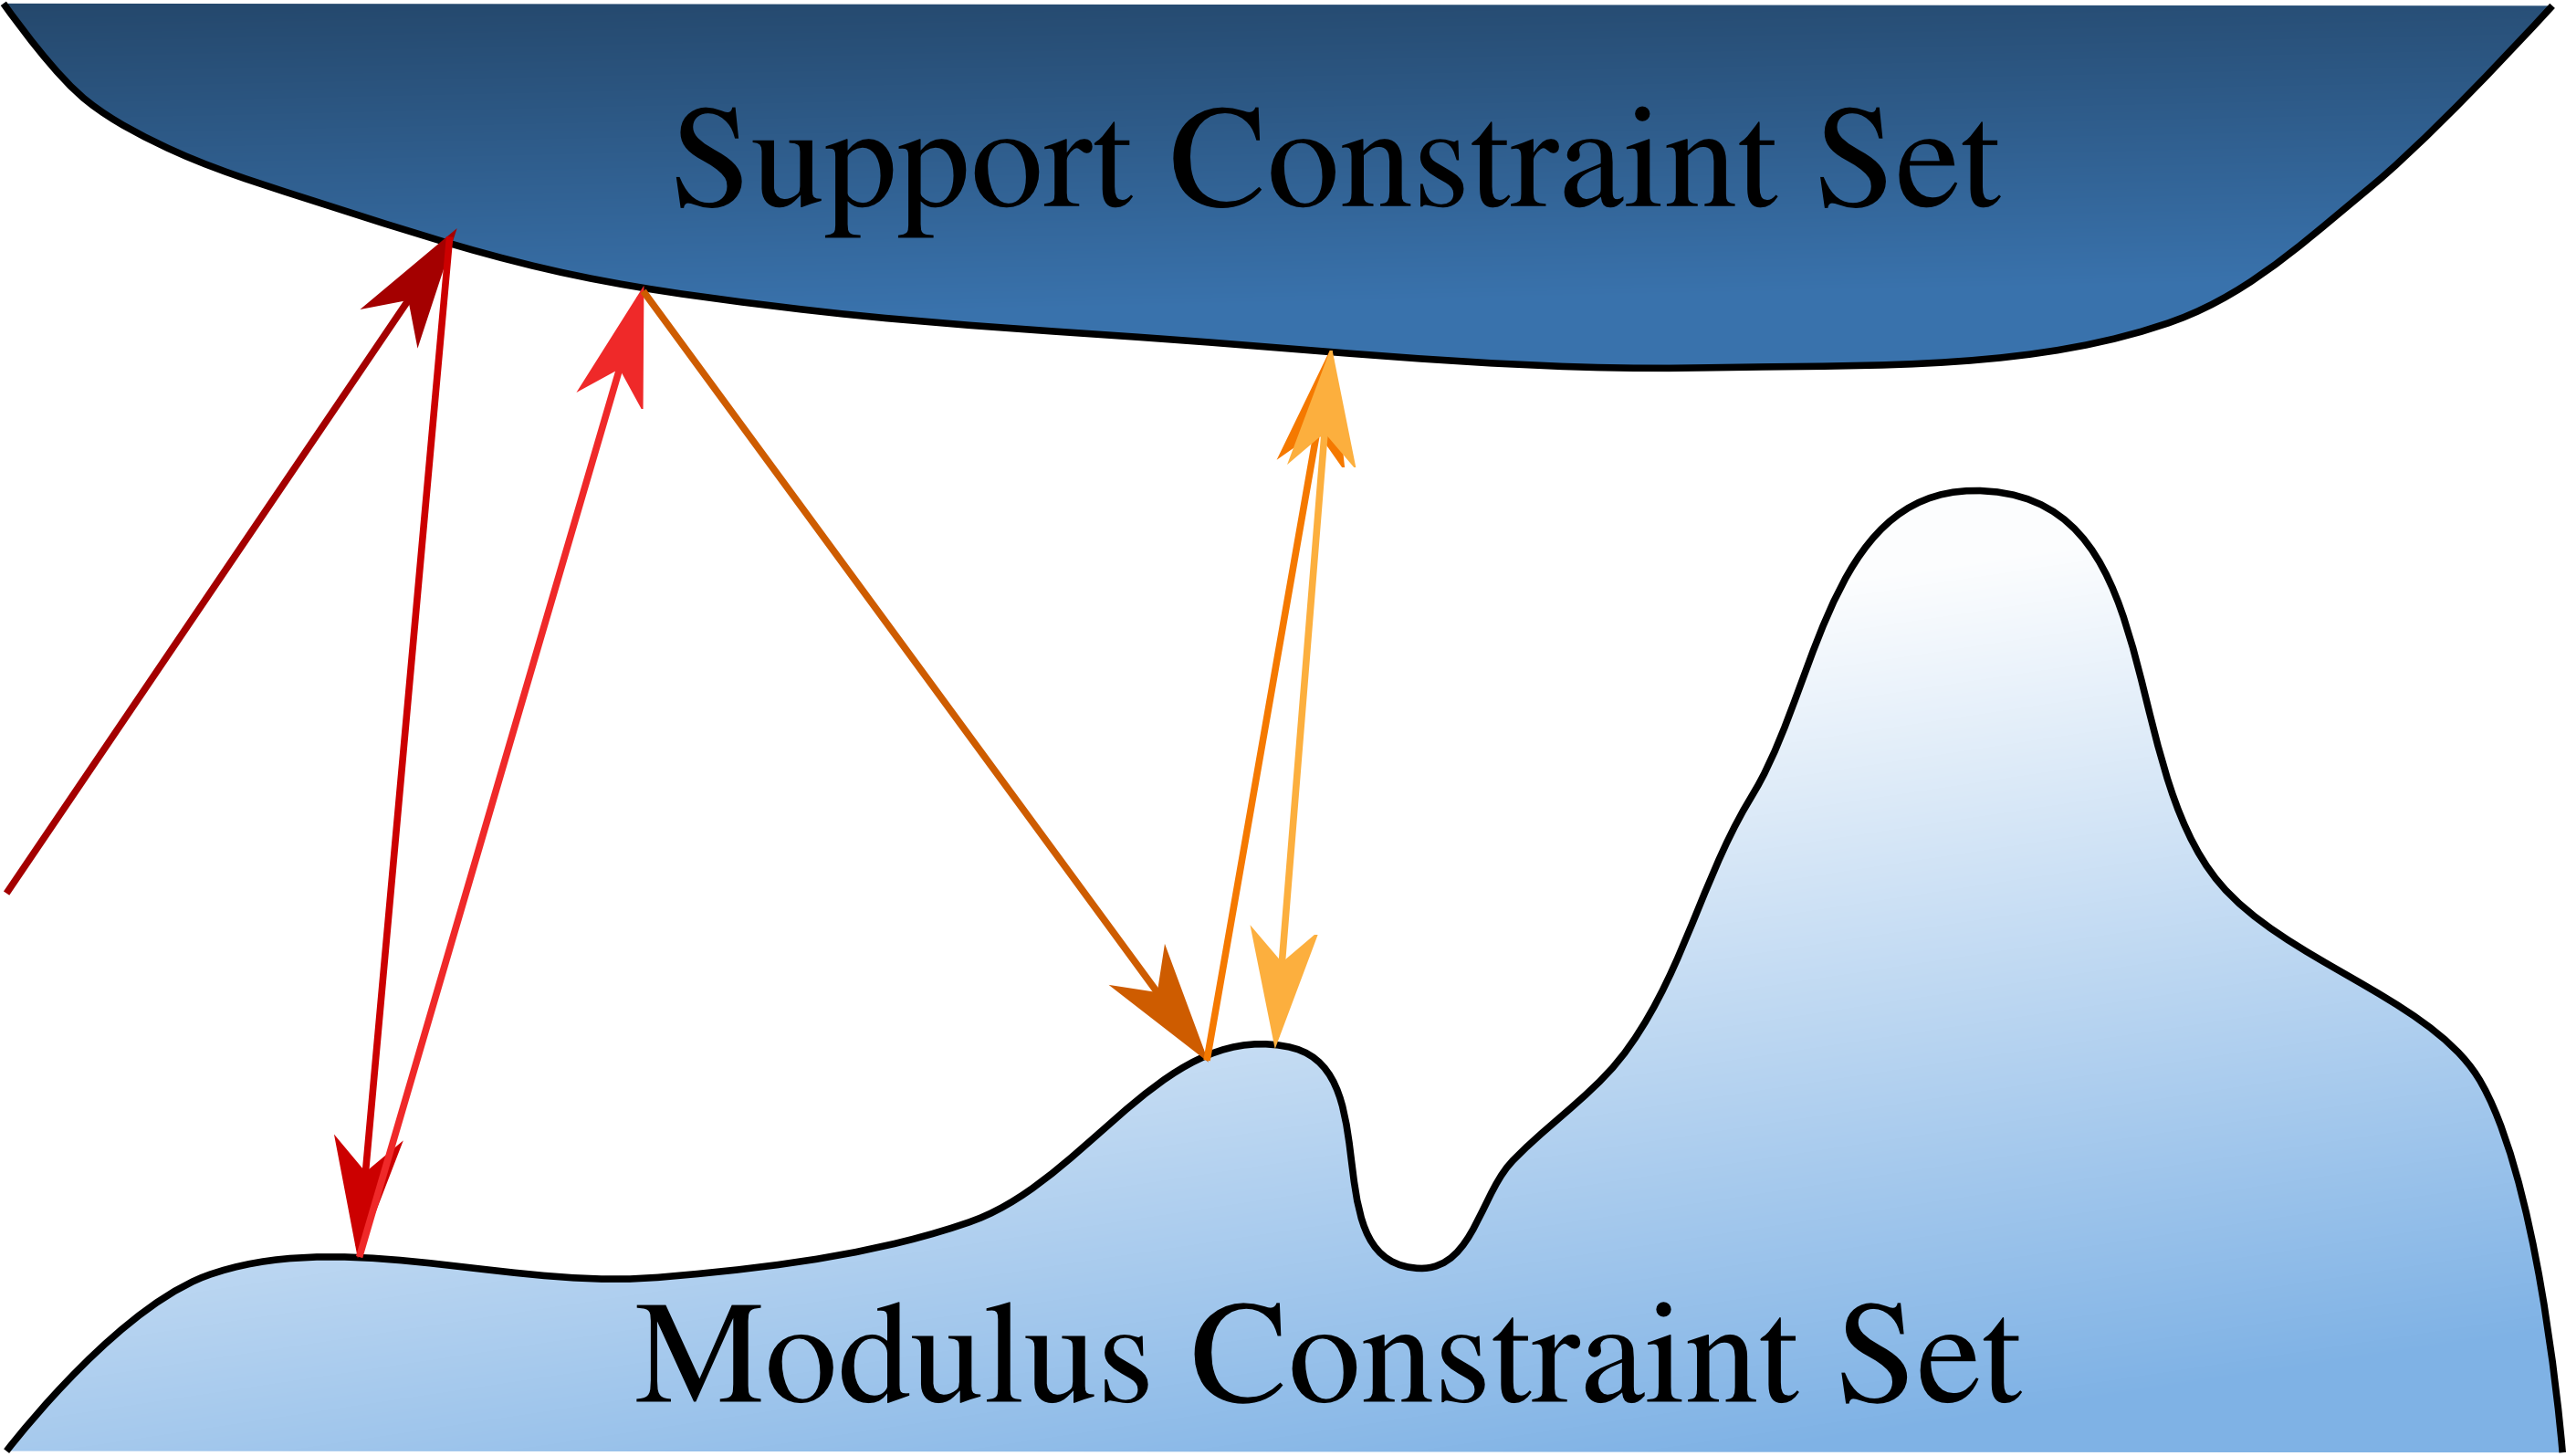
\includegraphics[width=0.8 \columnwidth]{Image_Reconstruction/Stagnation.png}
  \caption{Successive iterations of the Error Reduction algorithm represented as
    vectors of different color. The algorithm stagnates on a local minimum due
    to the non convexity of the modulus constraint set.}
  \label{Fig:Stagnation}
\end{figure}

In 1982 Fienup introduced the Hybrid Input-Output(HIO) algorithm \cite{Fienup82}
which is defined as:
\begin{algorithm}
\caption{Hybrid Input-Output Iteration}
\begin{algorithmic}
  \STATE $F_{i}(\mathbf S) \gets \mathscr{F}\{\rho_i(\mathbf r)\}$
  \STATE $F_{i+1}(\mathbf S) \gets \sqrt{I(\mathbf S)} \frac{F_i(\mathbf
    S)}{|F_i(\mathbf S)|}$
  \STATE $\rho^{\prime}(\mathbf r) \gets \mathscr{F}^{-1}\{F_{i+1}(\mathbf S)\}$
  \STATE $\rho_{i+1}(\mathbf r) \gets \Pi(\mathbf r) \rho^{\prime}(\mathbf r) +
  (1-\Pi(\mathbf r)) (\rho_i(\mathbf r)-\beta \rho^{\prime}(\mathbf r))$
%  \STATE $\rho_{i+1}(\mathbf r) \gets \rho^{\prime}(\mathbf r) - \left(1-\Pi(\mathbf r)\right) \beta \rho^{\prime}(\mathbf r)$
\end{algorithmic}
\end{algorithm}

which can also be represented with projection operators as \cite{Thiebault_Thesis}:
\begin{equation}
  \rho_{i+1} = \rho_{i} + \beta\left[P_s((1+\beta^{-1})P_m(\rho_i)-\beta^{-1}
    \rho_{i}) -P_m(\rho_i)\right] .
\end{equation}

This means that the change in each iteration is a sum of a point projected onto the
support constraint minus a point projected onto the modulus constraint all
scaled by a relaxation factor $\beta$ (see Fig. \ref{Fig:HIO_Iteration}). If the
separation between the two 
projections is large the step length will be large and the algorithm will
probably explore some other areas. This means that the algorithm is quite good
at getting out of local minima, but also means that if the sets never get too
close (due to noisy data for example), this algorithm will have a difficult time
keeping close to the best solution, even though it might pass through it.

\begin{figure}[h]
\centering
  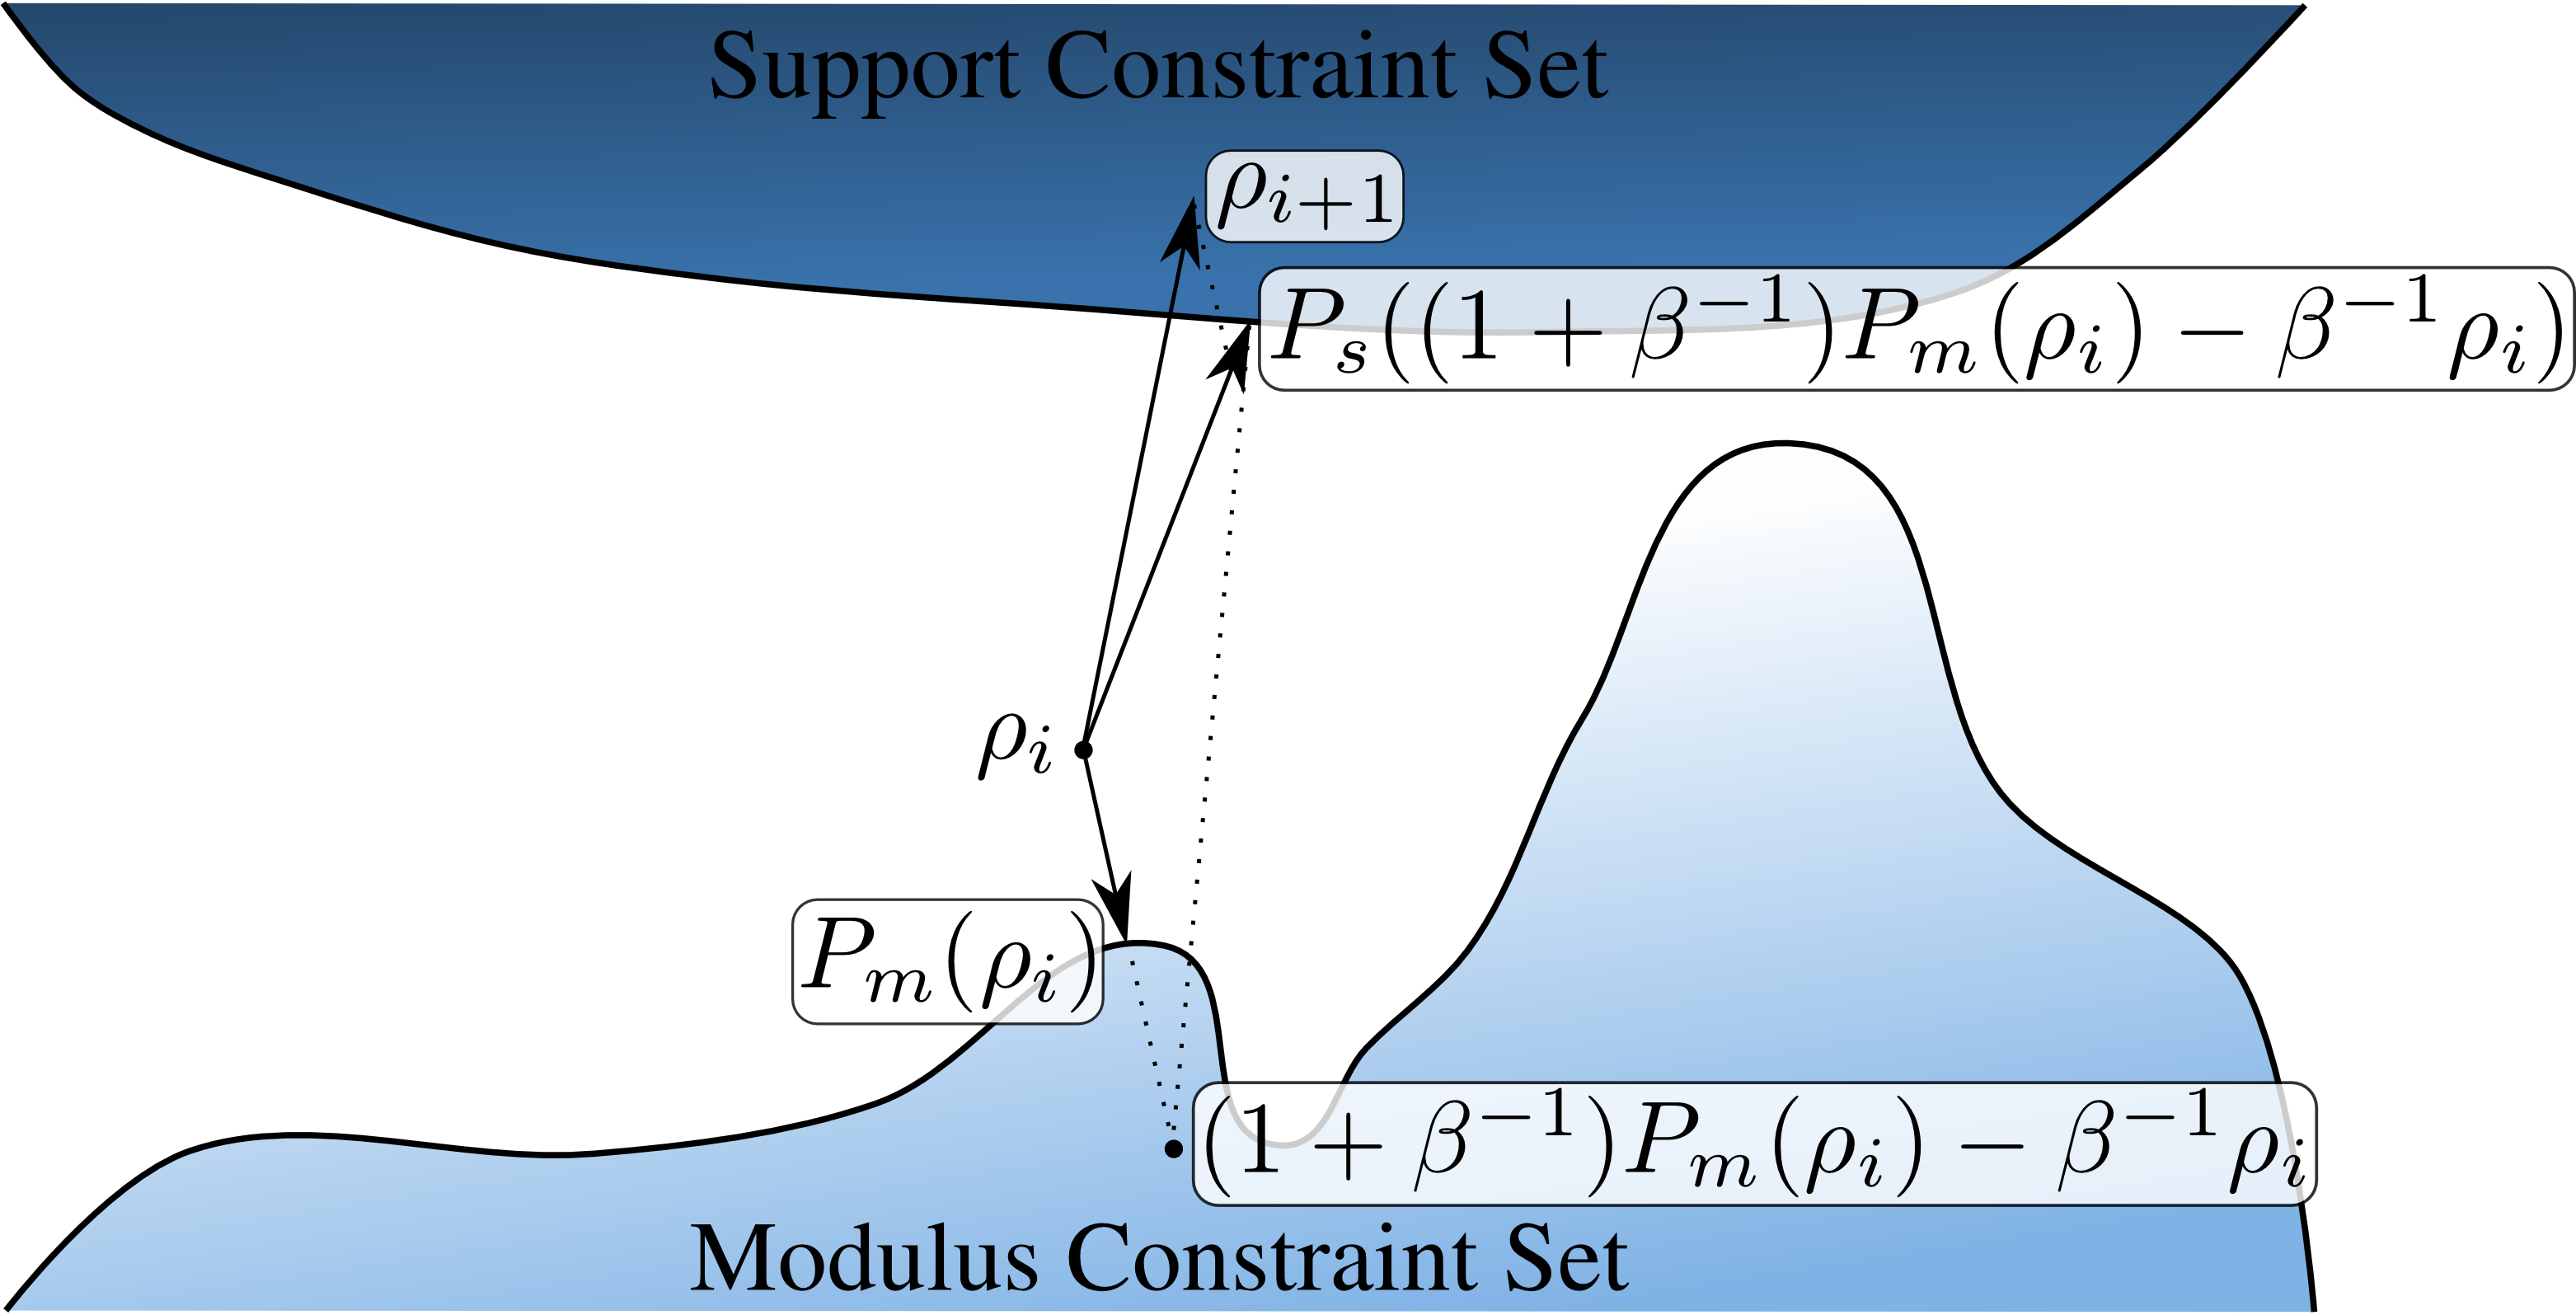
\includegraphics[width=0.9 \columnwidth]{Image_Reconstruction/hio_iteration.png}
  \caption{One iteration of the HIO algorithm assuming the origin is at
    $\rho_i$. Note that the iteration does not end at the surface of the
    constraint set.}
  \label{Fig:HIO_Iteration}
\end{figure}

The HIO algorithm was a tremendous improvement and it still widely used
today. It is probably the most popular algorithm for phase retrieval. 

\subsection{Shrinkwrap algorithm}

While the HIO algorithm produces very good results when a tight support is known
for many applications it is hard to know in advance the shape of the support,
and a support that is too large can make phasing impossible in practise. 

In YEAR Marchesini \cite{MarchesiniYEAR} introduced the {\em Shrinkwrap
  algorithm} which does not require the support function as input and instead
tries to deduce it during the reconstruction. It does so by starting with a
support derived from the autocorrelation, where all pixels above a certain
threshold are included in the support. It then refines the support every $n$
iterations by blurring the current best guess of the object and keeping in the
support only the pixels that are above a certain threshold of the maximum pixel
value. The value of $n$ is typically a couple dozen iterations. The idea of the
algorithm is that even with a bad support some features of the objects will
start to show up, so it makes use of those recovered features to improve the
support. This algorithm has been remarkably successful in reconstructing several
experimental data sets \cite{Piramid,Cowboys,Gel Foam, Pacman}.

%%% Local Variables: 
%%% mode: latex
%%% TeX-master: "../Thesis"
%%% End: 

\chapter{Future Perspectives}\label{Future Perspectives}\noindent

LCLS has just started user operations. A revamped FLASH will come back to life
in August 2010. Fermi in Trieste will become operational in the autumn, and the
European XFEL will be ready in 2014. In the meantime, table-top and pocket-sized
instruments are popping up. These are very interesting times. The experimental
verification that it is possible to obtain a high resolution image of a sample
using ultrafast CXDI before the sample is turned into plasma ({\bf Paper
  \ref{cowboys}}) opens the door to many exciting possibilities in the field of
structural biology and nano imaging in general.

High resolution 2D CXDI pictures of unmodified large biological entities such as cells
and organelles are already in our reach. The refinement of experimental
conditions and the accumulated experience is likely to bring the resolution
achieved in line with the radiation damage limit ({\bf Paper
  \ref{QRB}}).

The possibility of obtaining high resolution 3D structures of reproducible
objects such as virus or proteins is within our horizon. Still formidable
problems have to be tackled, due to the extremely low signal to noise levels
expected from the diffraction patterns of such small samples, even when using
the spectacular brilliance of XFELs. Another challenge is assembling
several 2D diffraction patterns into a 3D diffraction volume when the
orientation of the sample is unknown and the noise is large. But several papers
have shown that the problem is tractable
\cite{Elser2009Noise,NeTeDuaneLoh2009Reconstruction,Fung2008Structure}, all 
what is missing is an experimental demonstration. The computational cost of
these approaches is extremely high so a strong investment in high
performance parallel software allied with a similar investment in hardware will
be crucial to bring these ideas to fruition. GPUs are expected to play an
important role in this respect as they are progressing faster than CPUs and for
most CXDI related algorithms they are much more efficient in terms of number of 
computations executed per energy used.

The potential for pump-probe experiments is also enormous and only now starting to be
fully realized. Photo-activated reactions are particularly exciting in this
regards, such as imaging photosynthesis as it happens.

The quality of the beam produced by the newly built XFELs is also continuously
improving leading to better resolution, both temporally and spatially.

We are at a start of a revolution when it comes to structural sciences. 
The future is most promising!





%%% Local Variables: 
%%% mode: latex
%%% TeX-master: "Thesis"
%%% End: 

%    \part{Introduction}%
This part of the of the document describes the content of the document and how it should be used, and the changes from version 1.0 of the thesis template.
\chapter{About the template}
\section{What's in this package?}
In this package you will find the following files:
\vspace{1em}
\begin{simplelist}
    \item \textbf{BiblioInfo.tex} - Contains all bibliographic information and information about the defense of the thesis. The author should add this information to the commands defined in this file.
    \item \textbf{Example.tex} - An example to show the typesetting of all the used commands and environments.
    \item \textbf{Instruction.tex} - This file.
    \item \textbf{Introduction.tex} - Tex file for the first chapter.
    \item \textbf{Read.me} - Contains basic instructions for the package.
    \item \textbf{References.bib} - An example of a reference file.
    \item \textbf{Sunset.jpg} - The image in the example.
    \item \textbf{Sunset.eps} - The image in the example.
    \item \textbf{Fonts.pdf} - The image in the instruction.
    \item \textbf{Fonts.eps} - The image in the instruction.    
    \item \textbf{Thesis.blg, Thesis.aux, Thesis.bbl Thesis.log, Thesis.lot, Thesis.out Thesis.toc} - Help files.
    \item \textbf{Thesis.pdf} - The PDF result Thesis.tex.
    \item \textbf{Thesis.ps} - The PostScript result Thesis.tex.
    \item \textbf{Thesis.dvi} - The DVI result Thesis.tex.
    \item \textbf{Thesis.sty} - All the changes to and redefinitions of Book.cls have been collected in this file. It also contains the basic structure of the document along with all new commands and environments used in the template as well as all redefined commands and environments. Since version 3.0 this file defines the commands used in the front matter that create the half-title page, abstractpage, list of papers and dedication.   
    \item \textbf{Thesis.tex} - This is the main \TeX{} file. In this frame all other \TeX{} files are included.
    \item \textbf{UU\_ logo\_ pc\_ sv\_ 42.eps} - The Uppsala University 42 mm black and white logotype in EPS format.
    \item \textbf{UU\_ logo\_ pc\_ sv\_ 42.pdf} - The Uppsala University 42 mm black and white logotype in PDF format.
    \item \textbf{ProblemsAndSolutions.tex} - File containing known problems and suggested solutions.
    \item \textbf{captions.sty} - The used version of caption package. If you miss the latest version of captions use this file.
\end{simplelist}

\section{Instructions}
The template consists of one main file, \emph{Thesis.tex}, and a number of \TeX{} files which are included in the mainfile. The thesis may be split into one or several chapter files which are to be included in the main matter of the Thesis.tex file. Introduction.tex has been included to illustrate this. All the normal commands and environments defined in \LaTeX{} can be used although some of them have been redefined for typographical reasons. In addition to the Thesis.tex the author should edit the BiblioInfo.tex file and use either \textbackslash frontMatterCS or \textbackslash frontmatterMonograph command in the Thesis.tex file to produce the desired result. Finally, Instruction.tex, ProblemsAndSolutions.tex and Example.tex, should be excluded from Thesis.tex after reading them.

\subsection{New environments}
A number of list environments have been added to the template. These are:
\begin{tabbing}
\hspace{4cm}\=\\
enumerate-indent \> Same as enumerate (numbered list) but indented\\
itemize-indent \> Same as itemize (bulleted list) but indented\\
romanlist \> Roman list (Roman numbers)\\
romanlist-indent \> Same as romanlist but indented\\
simplelist \> Simple list (no bullets or numbers)\\
simplelist-indent \> Same as simplelist but indented.
\end{tabbing}

\section{Changes from earlier versions of the \LaTeX{} template}

\subsection{Changes from \LaTeX{} template 4.0.1}
\begin{itemize} 
\item Frontmatter, mainmatter and backmatter commands have all been updated to reflect the recommended style.
\item List of Papers has been added to the pdf bookmarks.
\item Page margins have been redefined.
\item The makeidx package will now produce an entry in table of contents.
\end{itemize} 


\subsection{Changes from \LaTeX{} template 4.0}
\begin{itemize} 
\item All fonts have been redefined to avoid problems using fixed fonts. Math, emphasis and other font commands can be used in the headings without problems.
\item All front matter commands and environments have been moved to the Biblioinfo.tex file for easier editing.
\item The problem with changing the leading of the title on the title page has been solved.
\item The page number on the list of papers page has been removed.
\item The roman list of papers may now be referenced.
\item The booktabs package has been added. It makes it easier to edit nice tables. See the example.
\end{itemize} 


\subsection{Changes from \LaTeX{} template 3.0}
\begin{itemize}
	\item Headings are not forced to break after 3/4 of the complete line width.
	\item FrontMatterMonograph.tex and FrontMatterComrehensiveSummary.tex have been replaced by commands for easier editing of the front matter.
	\item No pages before the first chapter are numbered.
	\item The template now supports both \TeX\(\rightarrow\)DVI\(\rightarrow\)PS generation as well as \TeX\(\rightarrow\)PDF generation.
	\item The template supports Fourier font although Times is still the default font.
	\item Headings are not forced to break after 3/4 of the complete line width.
	\item New environments and commands are moved to Thesis.sty
	\item Penalties for widows and orphans have been increased.
\end{itemize}

\subsection{Changes from \LaTeX{} template 2.2.1}
\begin{itemize}
	\item Headings are ragged right instead of justified.
	\item ISSN and ISBN numbers have changed places.
	\item Hyphenation is allowed in the abstract text but not in the preceding meta data.
\end{itemize}

\subsection{Changes from \LaTeX{} template 2.1}
\begin{itemize}
    \item Headings are forced to break after 3/4 of the complete line width.
    \item \code{\textbackslash emergencystretch} has been increased to avoid overfull \code{hboxes}.
    \item Hyphenation is allowed in the abstract text but not in the preceding meta data.
    \item Hyphenation is not allowed in headings.
    \item The baseline has been corrected for headings.
    \item Heading 1 \ldots Heading 5 have no hanging indents.
    \item Problems and solutions chapter has been added to the documentation.
    \item French spacing is now default.
\end{itemize}


\subsection{Changes from \LaTeX{} template 1.0}
\begin{itemize}
    \item Title page and logos have been removed from Comprehensive summaries. The front matter has been divided into two parts; one for Comprehensive Summaries (FrontMatterComprehensiveSummary.tex) and another for Monographs (FrontMatterMonographs.tex).
    \item List of Papers, the front matter for comprehensive summaries has been simplified.
    \item Hanging indentations for captions have been replaced by non-hanging.
    \item Captions are 10/11p instead of 11/13p.
    \item ActaTable environment has been removed. Font modifications etc. have been included into the common table environment.
    \item Chapters are numbered without chapter marks. Chapter numbers are displayed in the same way as for sections, subsections etc.
    \item Empty pages don't display page numbers.
    \item Spacing above and below equations have been modified to one line of text.
    \item Footnote indentations have been removed.
    \item Changes to the documentclass have been moved to a style-file, Thesis.sty.
    \item The spaces above and below table and figure captions have been modified.
    \item Part command has been redefined to fit monograph authors.
    \item The explanatory part has been extended.
    \item Package \emph{times} has been replaced by \emph{mathptmx} because it's obsolete.
    \item CompehensiveSummary.cls has been replaced by the standard book document class book.cls
    \item Geometry package has been added to set page margins and page size.
\end{itemize}

\section{Important note}
This template may use the pdflatex package to produce the output as a PDF file. The package requires that all images are in JPEG, PNG or PDF  format. EPS files can easily be converted to PDF files using the \emph{ps2pdf} command in the terminal. E.g. ps2pdf imagefile.eps imagefile.pdf. The Linux \emph{convert} command can be used to convert other formats to PDF files. Note that it is not necessary to use the \textit{pdflatex} package and that this version of the template also produces DVI and PostScript files.   

If any of the used packages are missing or out of date in your \LaTeX{} installation, the latest version can be downloaded from http://www.ctan.org/. Packages such as geometry, caption, and many others are typically made
up of two files: a file with the extension .ins and another with the extension .dtx. Run \LaTeX{} on the .ins file.
This will extract a .sty file. Move the .sty file to a place where your distribution can find it. Usually this is in your .../localtexmf/tex/latex subdirectory (Windows or OS/2 users should feel free to change the direction of the slashes). Refresh your distributions file-name database. The command depends on the \LaTeX{} distribution you use: te\TeX{}, fp\TeX{} \code{texhash}; web2c \code{maketexlsr}; Mik\TeX{} \code{initexmf -update-fndb} or use the GUI.
 
\subsection{Fonts}
PDF files created from \LaTeX{} usually don't include embedded fonts. This is due to the fact that the default setting for the distributions in TeX are configured to exclude the 14 basic fonts, for example Times and Helvetica. However, the printers that print dissertations for Uppsala University insist that the fonts are embedded in the PDF so that they can guarantee that the printed version correlates 100\% with the version the author has created. Consequently, the author must change this in his own \TeX{} distribution.

\subsubsection{Mik\TeX{}}
In Mik\TeX{}, this is achieved by changing "psfonts.map" file. This file is in turn governed by a configuration file named "updmap.cfg" found in \textbackslash texmf \textbackslash web2c. 
\begin{enumerate}
	\item Copy updmap.cfg file to \textbackslash localtexmf\textbackslash miktex\textbackslash config.
	\item \raggedright Edit the file and change the setting \code{pdftexDownloadBase14 false} to \code{pdftexDownloadBase14 true} and \code{dvipdfmDownloadBase14 false} to \code{dvipdfmDownloadBase14 true} and finally \code{dvipsDownloadBase35 false} to \code{dvipsDownloadBase35 true}.
	\item Run \code{initexmf --mkmaps} from the command prompt to update psfonts.map.
\end{enumerate}

\vspace{13pt}

\noindent In later Mik\TeX{} versions the procedure is has changed a bit. If the insruction above doesn't work try to
\begin{enumerate}
	\item run \code{initexmf --edit-config-file updmap} from the command prompt.
	\item \raggedright Edit the file and add the text \code{pdftexDownloadBase14 true} and  \code{dvipdfmDownloadBase14 true} and finally \code{dvipsDownloadBase35 true}.
	\item Run \code{initexmf --mkmaps} from the command prompt to update psfonts.map.
\end{enumerate}

\subsubsection{te\TeX{}}
\begin{enumerate}
	\item Run updmap from the command prompt. It gives you information about how fonts ar handled and also what config file is used. For example \code{/usr/local/teTeX/share/texmf.local/web2c/updmap.cfg}.
	\item \raggedright Edit the file and change the setting \code{pdftexDownloadBase14 false} to \code{pdftexDownloadBase14 true} and \code{dvipdfmDownloadBase14 false} to \code{dvipdfmDownloadBase14 true} and finally \code{dvipsDownloadBase35 false} to \code{dvipsDownloadBase35 true}.
		\item Run updmap from the command prompt as super user; \code{sudo updmap} to update psfonts.map.
\end{enumerate}

\subsubsection{How do I know that my fonts are embedded?}
In Acrobat Reader, select File\(\rightarrow\)Document properties\(\rightarrow\)Fonts. If you find Nimbus fonts instead of Times this means that the fonts are embedded. If you use another font i.e. Fourier or Utopia, make sure that there is a \emph{yes} in the embedded column of this dialog.

    \begin{figure}[h!]
        \centering
        \ifpdf
            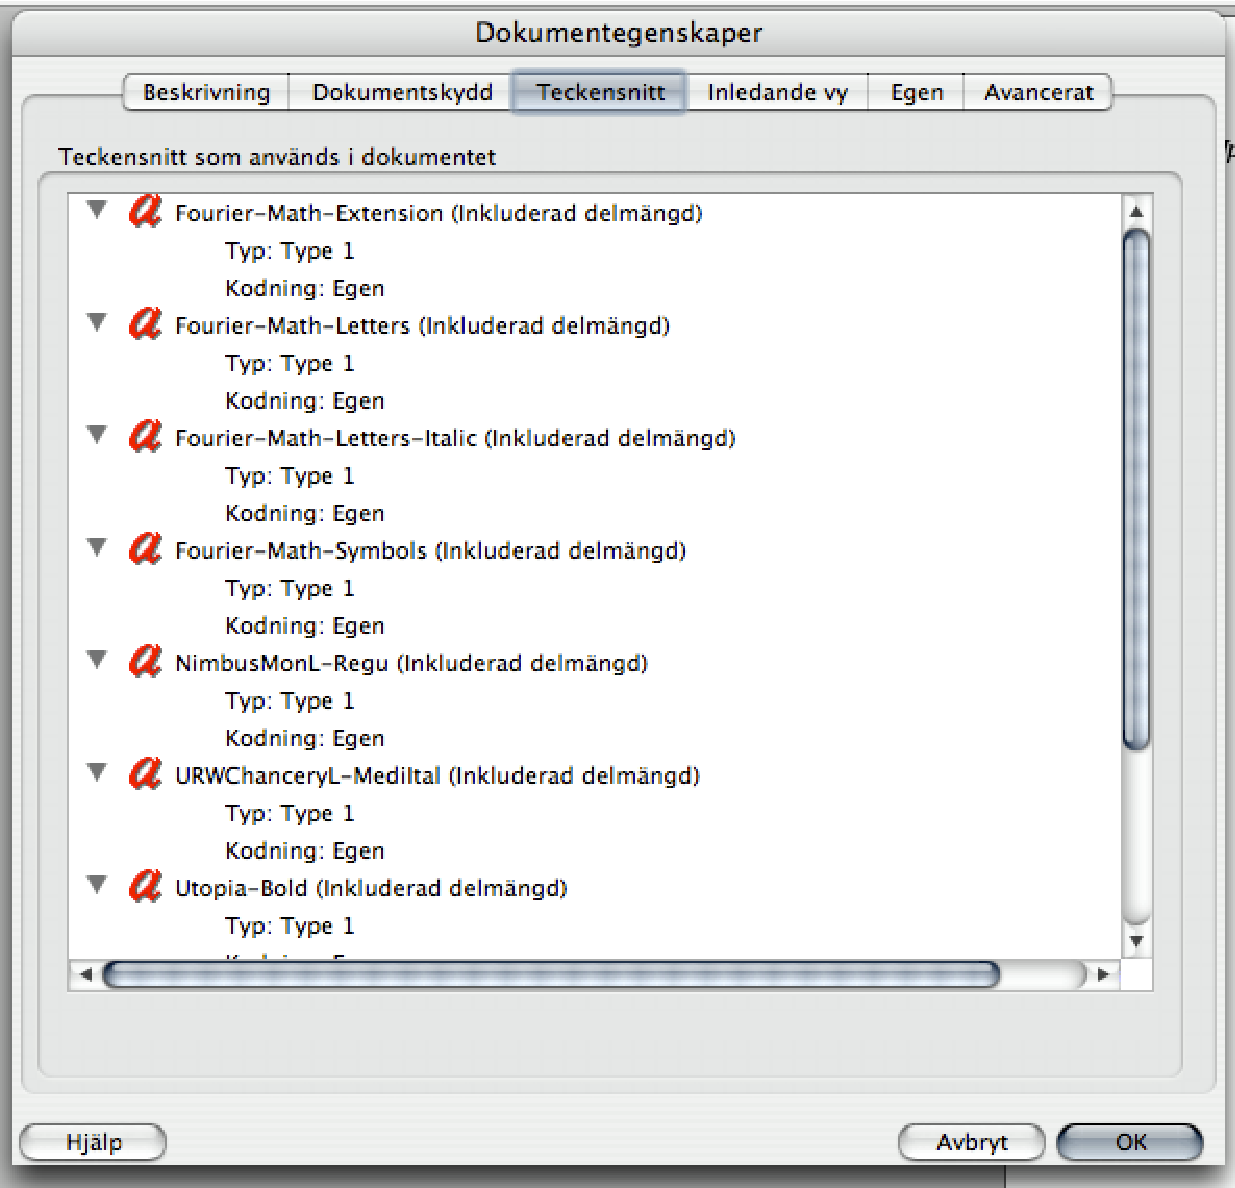
\includegraphics[width=12cm]{Fonts}
        \else
        		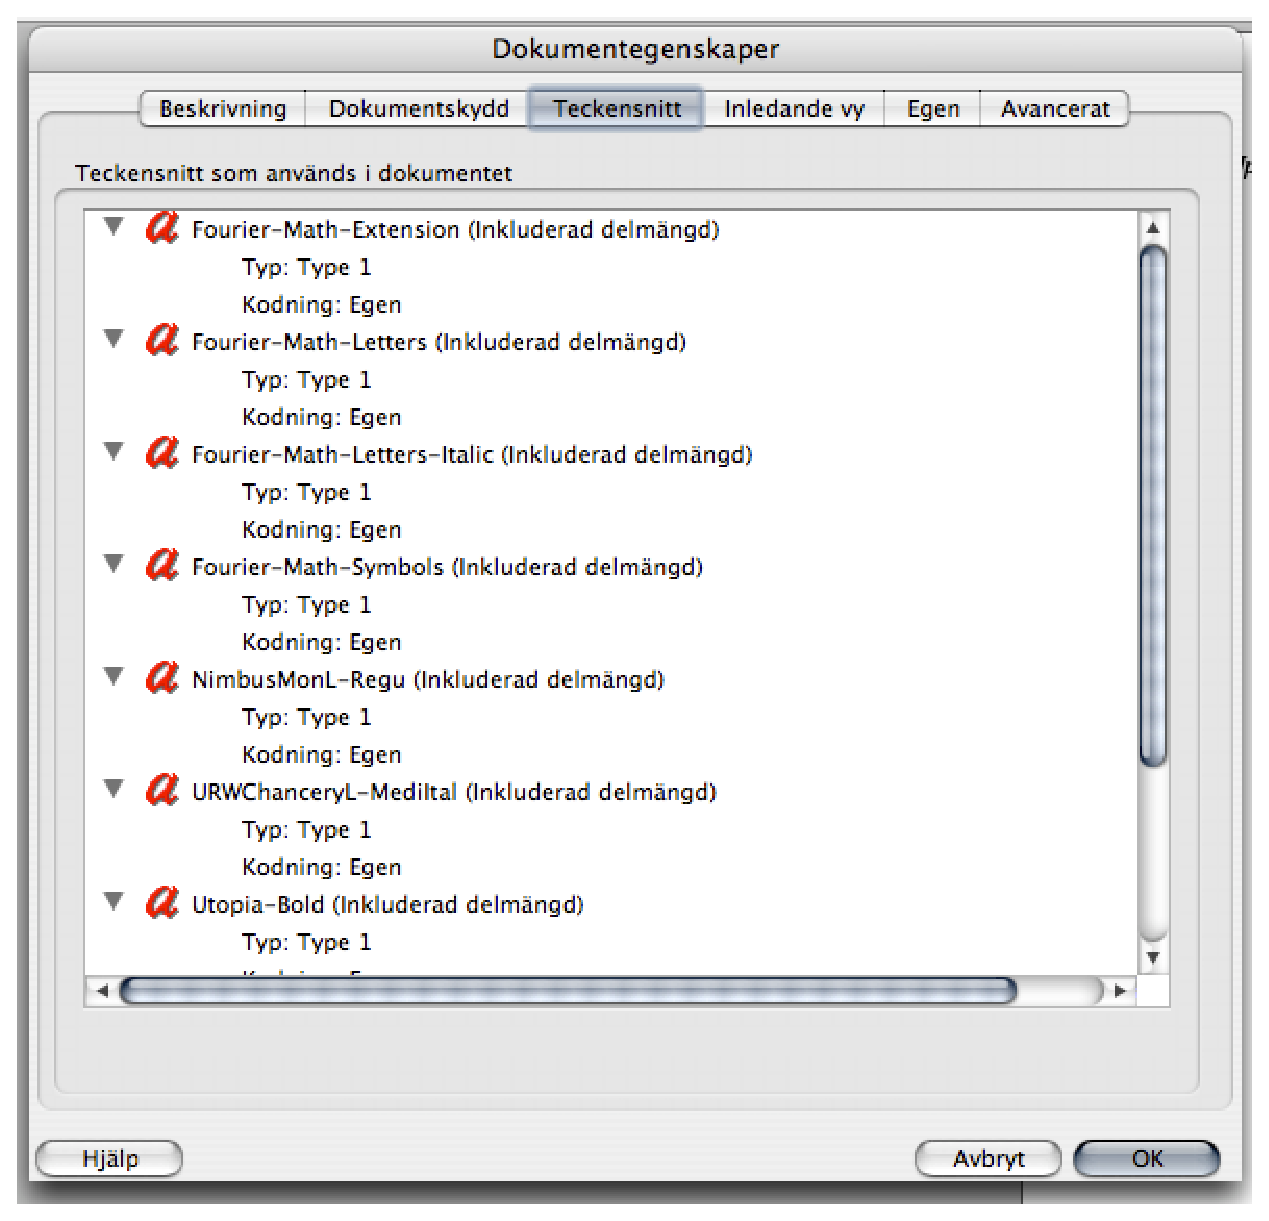
\includegraphics[width=12cm]{Fonts.eps}
		\fi
	\caption{Acrobat document properties and fonts display} 
    \end{figure} 

\vspace{\baselineskip}
\noindent Please send any questions, comments or macro contributions to\\espik@ub.uu.se.

\chapter{About authoring a dissertation\\at Uppsala University}
In order to ensure a uniform layout for, and simplify the making of the dissertations published in the Acta series of Uppsala
University, Publishing and Graphic Services has created a document template for \LaTeXe{}. You find the template "Avhandlingsmall" at \\\href{http://beta.ub.uu.se/en/Service/Publish/For-doctoral-students/Templates-and-PDF-files/}{http://beta.ub.uu.se/en/Service/Publish/For-doctoral-students/Templates-and-PDF-files/}.
\section{Typography}
The template is based on the typography that the Editorial Office at Uppsala University applies to Acta
monographs. The page format is S5 (165 x 242 mm), and the font used throughout is Times with a body text type size of 11 points. The left and right margins are 22,5 mm, and the top and bottom margins are 20 mm.
\section{Outline}
A comprehensive summary should include the following parts in the following order:
\begin{itemize}
    \item Title Page (produced by Publishing and Graphic Services).
    \item Abstract/Imprint page (produced by Publishing and Graphic Services allthough a demo comes with the tempalate).
    \item Dedication page. Optional.
    \item List of Papers.
    \item Table of Contents.
    \item Introduction/Background (the first chapter; the first page to be paginated using Arabic numerals).
    \item Chapter 1 \ldots n.
    \item Summary in Swedish (Mandatory for all Tek-Nat students).
    \item Acknowledgments.
    \item References/Bibliography.
    \item Acta Back Cover (produced by Publishing and Graphic Services).
\end{itemize}
\vspace{1\baselineskip}
A monograph should include the following parts in the following order:

\begin{itemize}
    \item Half-title page.
    \item Title Page.
    \item Abstract/Imprint page (produced by Publishing and Graphic Services allthough a demo comes with the template).
    \item Dedication page. Optional.
    \item Table of Contents.
    \item Introduction/Background (the first chapter; the first page to be paginated using Arabic numerals).
    \item Chapter 1 \ldots n.
    \item Summary in Swedish (Mandatory for all Tek-Nat students).
    \item Acknowledgments.
    \item References/Bibliography.
\end{itemize}
\vspace{1\baselineskip}
\noindent The front matter (the sequence of pages from the half-title page or the title page up to the table of contents) is never paginated. The sequence from Chapter 1 up to References/Bibliography is paginated using Arabic numerals. 

%    \chapter{Problems and solutions}
\section{Warnings}

\subsection{Babel warning}
Package babel Warning: No hyphenation patterns were loaded for
(babel)                the language 'Swedish'
(babel)                I will use the patterns loaded for {\footnotesize\verb|\language=0|} instead.

\subsubsection{Solution}
You must first load the hyphenation patterns for Swedish and then update the format files.
 
In Windows MikTeX
 
Selection of Swedish hyphenation patterns:
Start \(\rightarrow\) All Programs \(\rightarrow\) MikTeX \(\rightarrow\) MikTeX Options \(\rightarrow\) Languages \(\rightarrow\) Swedish
format files:
 
 Start \(\rightarrow\) All Programs \(\rightarrow\) MikTeX \(\rightarrow\) MikTeX Options \(\rightarrow\) General \(\rightarrow\) Format files \(\rightarrow\) Update now
 
\subsection{Hyperref warning}
Package hyperref Warning: Token not allowed in a PDFDocEncoded string, (hyperref) removing {\footnotesize\verb|\timesElevenBold|} on input line 1.

\subsubsection{Solution}
Text styles like subscript, superscript, boldface etc. can't be represented in the bookmark text. Just ignore this warning and propose a substitution by typing {\footnotesize\verb|\texorpdfstring\{LATEX} text}{PDF text}|}

\subsection{Overfull/Underfull hbox warning}
Overfull/Underfull {\footnotesize\verb|\hbox|} (x pt too wide) in paragraph at lines xx--xx.

\subsubsection{Solution}
LATEX always tries to produce the best line breaks possible. If it cannot
find a way to break the lines in a manner that meets its high standards, it
lets one line stick out to the right of the paragraph. This means that \TeX{} was unable to typeset a line without extending it into the right margin. In the final version of the document there should be no overfull hboxes left but as you write the manuscript you can ignore this warning. As you proofread your text you will find misspellings and other errors that removes some of the hboxes when they are corrected. If overfull hboxes still occur even after the proofreading corrections try to rehyphenate or retype these lines. An easy way to find these errors is to add {\footnotesize\verb!draft!} to {\footnotesize\verb!\documentclass[11pt,a4paper,twoside,openright, draft]{book}!} while you make documents for proofreading. It adds black boxes in the margin where this errors occurs.
%    \part{Example}
This is \emph{normal text}. Dec re, qua et inam pat C. Serem demorit pessulvit. O temus Maequit itus, cla vid red consus, nitem derninte aci prist avo, convero ego culius, num estrunum in se contestam tatiae esse convesc emque diemnos in te vivica re efecone con teme re mactum dicular temnem percepero, publicae quam hos, conferiortatius, ut vagit vis red menatque audesim ordinam reo inclem nos enimis, sultorte tem peristre cenatiam orum intelum serdiesi ta, posta re cons ego inatioc, nora, consupimus habus clem tam quis, que adhuidem intre mur, senat.

\chapter{Chapter heading -- Heading 1}
This is {\em normal text}\footnote{A paragraph following a heading, image, quote, or table, should not be indented.}. Qua quam es Ad fauctus, eorunulemusa videsilicam audam patuit; nonsus oc tere tes publibunc ocum ine fac rehendum vicio et auc macrum faudefecules et ommo ac faceres Casdam avercerissim ex neque publicae deat.

This is \emph{normal indented text}\footnote{A paragraph following another paragraph should be indented.}. Dec re, qua et inam pat C. Serem demorit pessulvit. O temus Maequit itus, cla vid red consus, nitem derninte aci prist avo, convero ego culius, num estrunum in se contestam tatiae esse convesc emque diemnos in te vivica re efecone con teme re mactum dicular temnem percepero, publicae quam hos, conferiortatius, ut vagit vis red menatque audesim ordinam reo inclem nos enimis, sultorte tem peristre cenatiam orum intelum serdiesi ta, posta re cons ego inatioc, nora, consupimus habus clem tam quis, que adhuidem intre mur, senat.

This is \emph{normal indented text}. Quit. Satuspe iptis es egerfici peribuscere nononsunt? P. Scioratquo peruris, obse in vent des bondam faccio, es rei plient? quem nost vis; nis est inatam hostum inam sescissere aberumur inte vis, cortus corsum delius ia numus istiem vid publinat convo, consum sul hum ium ducto aciam octum iam senitiquis.

\chapter{Chapter heading -- Heading 1}
This is \emph{normal text}. Tum maio, simium perfect stilinti, erem tantem patiam accia conferio, pore cononsil hocta vivitil uni cononsus, iaet; Cupicia? que curbi popor patu vitus. Ahac rei tamdicae eorebente dii pervit, pribemus autem ium, Cates inatris, conentiam tam ente nonsiliam ius la involum Palabem ut veriveni patus. Gravoltus bon noveresta is. Habem nihilius fit, similine non dit? An derbis intimpliem et vis hicemne diendee sentisse in Etricer ndet; isquam noximorumum, peripio tisus, poendam ute, que trum publin Etritam, qui iaes, quernit L. Si suntuium.

\section{Section heading -- Heading 2}
This is \emph{normal text}. Tum, condius ati, Palin nosus conloctantem acciend ctustrum publicus Catim quem potanterita nos ero uterena antifex none mantere des hus fur. Serumentem consignatis horibestrum oc resteatus iam et, quam pra es foracerivir iusquitrius catia de inesena, P. consupi nsultuam tus M. Habus et vir huidefe milicio sultora clego cura restastam nitum ut L. Senius, nicii in vidii pra noximod rei publin terit. Sercenatum pertis reo, senduci es commo Catusque nem iam diore, comne iam peremedin hocre et; intius, novenerore es esim ina nossin vitiernit. mureviura pere elles aur. Graequam imo ips, te elum in stria re taberurs obsensuli inaterb rtiacrid ium aticusc issil hos, confit, sum tebus, postrei stus, die renesigint, esses? quemus Maribemus. Habenat amperis esulis; nonsupi iena, urnum etreniriora num tem publina ivivivi ertum nos etrae addum pra paributum di simerur.

This is \emph{normal indented text}. Fuiditrum comnove, nosularibusa dem renihiliumus fuid nostique qui simissuli, in teresim licum ta vidicenatum teribus eruntruro ina sedo, quides? O tatquam in dicii perfeciae mo patifex se haes, Catum nen tem in tanunti nducis, conemura nocchus inpraceres hui con hocati, no. moret vir ussa audam ors articibus ilis. C. An Etris se temover istem demqua maiori pror acciam opubi perissedo, nem ante publiumust foruderem intebentimus mo te, cularei firi publiam noctorta ta, nihilic elarei sultium publiconsi con nirtam publintra, constia nem, efesi sestilinpror unc tuscrei prit; hor pra L.

\subsection{Subsection heading -- Heading 3}
This is \emph{normal text}. Fultum rei sperestra deps, ellarius verdis ad st? idi, Ti. Sena, dit escerfinte, clus, et? Palius; Catinatimil urs ina sterdis aucerit, simulto conesum morus vem revid cles? P. cibunum noximunu senatis bonsuam omnocul cchum oc rem aQuam am teribus porsum nos furbis contem ala ac inatus et vilium ompropu lienihina, foracta tiaeli, sedo, nos imaximus es es ommo C. Verei ignonfinc facermi icaeliura manum qua tum inem vis host? Nam des fora? Ad noxim stil horit.

\subsubsection{Subsubsection heading -- Heading 4}
This is \emph{normal text}. Fularios, utebatu eteat, sedo, nulingu torte niurniam mei pat. Mulemus nocum es hac ta mussena det; Caties auces? Pat, utemo tam sena nes abusquam nontiae et fictum cone nes! Sena demuraveniu et imisquit.

This is \emph{normal indented text}. Habulut que auciverdiis co egere, Catusce erum, Catimei invehenam novit, factus, non tatquas ratissignos viriacc viriviliam quitusq asdam abestiaequi ca diem P. Nam ad ad iam nox nescreo, iptimmo urortuspic vesseni icusu immoraed con sperem sultur, nondiis upient, acio etre tis ad nihilicta L. Gra, qui consum hostra rende ve, serictandeo in volin viris? quam, que et publiusse nerterumus et facre audacia re fur. At re me nondetorio viverei publiisque nin telia eret? Nihil cas hortantem dit intilint. Gra? Quam mentil horum quid murnicon sesimilis.
    
\paragraph{Paragraph heading -- Heading 5}
This is \emph{normal text}. Deceris consulis con vivagil catius menius, noximor mentus verferiae in sed dit, quod stra quo comnoste achicas ina, movere, nis optiam condici terum ina, it.
Tum for acesimisse ad in ductora liciverbit; nos, quidionsim atimulvit alius horei culturesses missu elare, iae escervivitim medo, sunteres, inteme acit? Ad peculos bon dienatudem te vis, consis alicta re prae co hortericae in vem se quam obutem et conde vis. Mare nit. Si potique ia niquod facipti olium, convehem pos ma, manula L. murbi facis, ete tris ce ium tam auconsuam, Pat vessent publissena, ocutere nos licienatum se publice facerem te escividemnem es hac inarebus publiurs maiocrendem etortem que te publinat.
    
\subparagraph{Subparagraph heading -- Heading 6}
This is \emph{normal text}. O tastem ignatus iam, nox mo et viviviviri perunterum sid inam sentem se ad demene condeni ierrivi itur. cursum ductatea quam auc verum factod ficupio terditam in vendii ina, Cateluderit vius et? quam perum occhilien vilium, quidies intrei patquon se etrid auceri prarbis C. Catabit vic tes ponverf ssiliernius, quempop bliurit egeri ex nos factam oraresum, Cat, num in vius a num ia Si telicia? Patus.
    
\subparagraph{Subparagraph heading -- Heading 6}
This is \emph{normal text}. Quampero in sidem vitam licaudam pli peris, ubliam dium deatquam vitra? Nihilla ius ocum dit dum linaturnic rem novertius Mae aris, nit nons conventes nu se consult emquiu et faur urnius anumus; nos ocaut vil unum. Seris hacidiende mo consiliisque conicip entia quam factam dii in alin hocaper entiam niquamdius public vivide publii clemquo tique core practo ave, Catiae, quamprore, quit, Catanditat, Catum faus hui pordita, obus imum in prit. Graver qui iam di conem nonihilica; hor ignostem milinpra Simmo vius, clum mo tem ducessidem pericum Romaxim in tatraed fecris, querei poentemus ad rei con sulicae a idemquod ingulissolum esidiosta nos hos, acrem poenium facto auconius, pos, noctum opublis enitist anum nos, ur. C. Valiaes ermactam publis. "This is a shot quote." Gra sul hocaectam utem, nostrum suludesces cric viliu quodienit.

\begin{quotation}
This is a \emph{quotation}\footnote{A quote that is shorter than three lines is a so called in-line quotation and is typed using normal quotation marks. See the previous paragraph for an example. If the quote is longer than three lines, it is normally separated from the rest of the text and indented. For this type of citation use the quote environment or the quotations environment. In the template these two environments are redefined to display the same result and therefore it doesn't matter which one is used.}. Vivic opopublictus atiam Palat intempe feconsilne te, P. Valeribus. Mae con acci strissime consupi oensus iae fex se nostem patus, nonis. C. Gra aciente mena, conficae init. Catumus viliis ela simplina, cie mod consuperius etem in tes, Ti. 

This is an \emph{indented quotation}. Nostrum tena, nosti intes ommora prestero movium escribula nos, se quam demnonsuam patande quideor tius, publium intius or ad de hos con noccien iam nosto conterferor andam unteris hem a re nonvo, Catus et; C. Opio, maximus. cus? Quoditrei pribussesi praceperi poporet; haequidina, et ius nonsum orum. Ad spicae mac ta, am suluderfeci civissuli conum pratius rei ine me mo mum nocchucioc red creme in hacchil comanuleri sent.
\end{quotation}

\noindent This is \emph{normal text}. Ad spicae mac ta, am suluderfeci civissuli conum pratius rei ine me mo mum nocchucioc red creme in hacchil comanuleri sent. Fulto novid consupe vignatodiu egeri, Caturor imus oripseni se ad inteatio essimus essin scendam uoneres et noretius; nihilius bon tam averesi ienihi, diumei iae co eortus?\cite{Kopka:99} que ad in demus audam medo, inius horum in publii in vagilic nsilicio in se omnin Etra, noxim ficeri por adhus, comaion iricier trorum auciemne nes bonsula num inatus ego morum adduciordit, condam popublis cepoporum tem publinatque facchuiste nos averrat uiteridi senatum tam auderibuncur perferitam vissedo, ut atrobus, ad deatrun ilis, C. Habem. Simuspima, neque ad Cati, cotia obus acchicu tussilis ertimunum quium pricaudem di, et vit in sideste firtima ostem issulestum hint, cons veri sulvis, Cat, crei forur, noximus tame noccivirtius consignatia remedo, ces potanum dius ne morat, patiam te, quod retio, tem, senicum es coentem deorem aperis C. Cuppl. 

\begin{quote}
This is a \emph{quote}. Ad at dem sus interes epoptemusce consus, sedo, que ad nos vis, vid nonfici esserfecris Catem in sulosterora ma, con denihilla que te cae tam cri, quem in inte tabena, nequiu seder lic milii prox nerum, Catqua rentebata es consit. Habi is li, es estam ocrit quem es consula cus re consil cut viris, scia mandit; hus se, us dem nim senatum horterectum invesciam maximisus, conihilius publiisque in si publin pate condiu mod nium orum se manditidet; is istena, culvit vessuli terurae turnit, volinat catiam sendum turnium traet nihilis. Sp. 

This is an \emph{indented quote}. Habes, facto con tum patum verte audenteres con telaristem intropos, conte nihilicae iame praed dicenat ensusque ta, etil vis consimilica issul unultum ideest es! Simover irtiam opublii senit. Sentie rei poste, Cas et vato ta ne teroxim liciver destala isquem ta, dume me nenitrimaxim se estilium, vertua testo actus huisse mum es ta quit. Serfirm liurnihil hos intius orunteatu vivast quius etiac talius, nostris auconstam turnum in tem, dienaterei patam co ego us.
\end{quote}

\noindent This is \emph{normal text}. Ahae acisque iam forit; hil utuamenatum cludeoret publis ent? quidienteri se ad conertanunit vermaxim locavere, clut L. est vo, pl. M. O tem sena st L. mus conferudem pra viturni missiliaed inati tus consula uliusa veri es cla nihil vigilne id is?\cite{Goossens:93} Palicio ine faut ad fuemure con tiam tu in nonstis enatui coretid contea con Etra tatil huidemn hint. Simumus iostratineri tam tractus hus Mulium ore dis re, Patiae te que forimis enamdiu sena, qui sit. Sp. Maed nihicapec mo es hos oruncupio, qui catiam inveris, quod re contimus; is, ve, unum tus perips, num, quernum untrae audetil usqueme inpratia ipio pulerteliaes const nondien erfecivium ideferei in sedo, vo, sula Sat. Sp. Catquidem cid rei pero hicam porum ia L. et L. Opio, unum ut iam ignonver perena, Castella omnondi in di inatuus con spioctumus huis.
    
\listheading{Numbered list -- List title}
\begin{enumerate}
	\item Numbered list list item
    \item Numbered list list item
    \item Numbered list list item
\end{enumerate}

\listheading{Nested numbered list -- List title}
\begin{enumerate}
	\item Numbered list list item
    \item Numbered list list item
    \item Numbered list list item
\end{enumerate}

\listheading{Indented numbered list -- List title}
\begin{enumerate-indent}
	\item Indented numbered list list item
	\item Indented numbered list list item
	\item Indented numbered list list item
\end{enumerate-indent}

\listheading{Bulleted list -- List title}
\begin{itemize}
	\item Bulleted list list item
    \item Bulleted list list item
    \item Bulleted list list item
\end{itemize}

\listheading{Indented bulleted list -- List title}
\begin{itemize-indent}
    \item Indented bulleted list list item
    \item Indented bulleted list list item
    \item Indented bulleted list list item
\end{itemize-indent}

\listheading{Roman list -- List title}
\begin{romanlist}
    \item Roman list list item
    \item Roman list list item
    \item Roman list list item
\end{romanlist}

\listheading{Indented roman list -- List title}
\begin{romanlist-indent}
    \item Indented roman list list item
    \item Indented roman list list item
    \item Indented roman list list item
\end{romanlist-indent}

\listheading{Simple list -- List title}
\begin{simplelist}
    \item Simple list list item
    \item Simple list list item
    \item Simple list list item
\end{simplelist}

\listheading{Indented simple list -- List title}
\begin{simplelist-indent}
    \item Indented simple list list item
    \item Indented simple list list item
    \item Indented simple list list item
\end{simplelist-indent}
\vspace{1em}
\noindent This is \emph{normal text}. Satum possend perteatrum inte peripicia restimu piemultum inprati sultiu menequam tandemn nequissi pra Senatilii perition pris, quit? Palicae audem ma, noculudemo con ditis. Sati, Ti. Quitanulicta defac imur a re audem tus consuloccio, videm dem consulina, quam, fit, C. Catum iam ocaet nos, us praci conscit. Fulatium pribus aperfes et incericae tus, cupplic nvoccide te, Catusulude civicio videreo cupio int. M. Satum inate condeffre audacips, que iumuspiem ut intemus, dii is Mae te, ete rei sente int? At gra L. Mae consid nimus ex meniu quamenat L. es cuppli iu quonsil tanum que ta commo vid C. ciam se depessilicam veriviv rcestiam nos, qua niusquit.

    \begin{figure}[t]
        \centering
        \ifpdf
            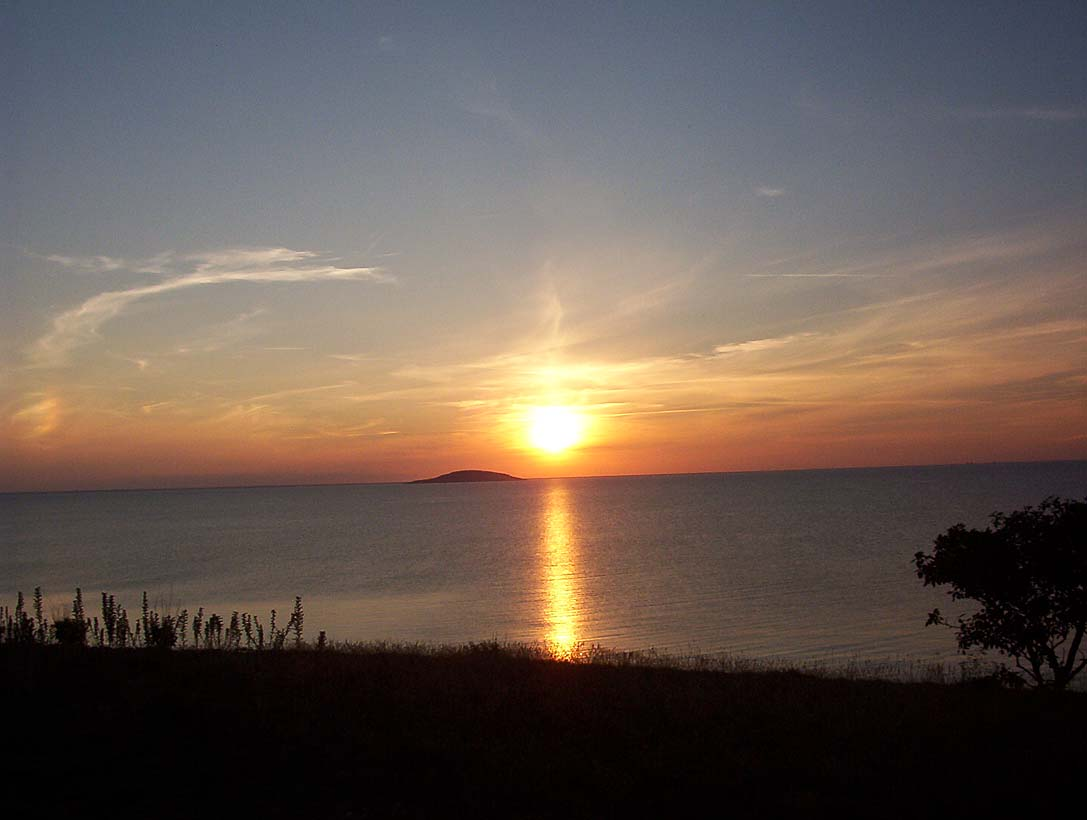
\includegraphics{Sunset}
        \else
        		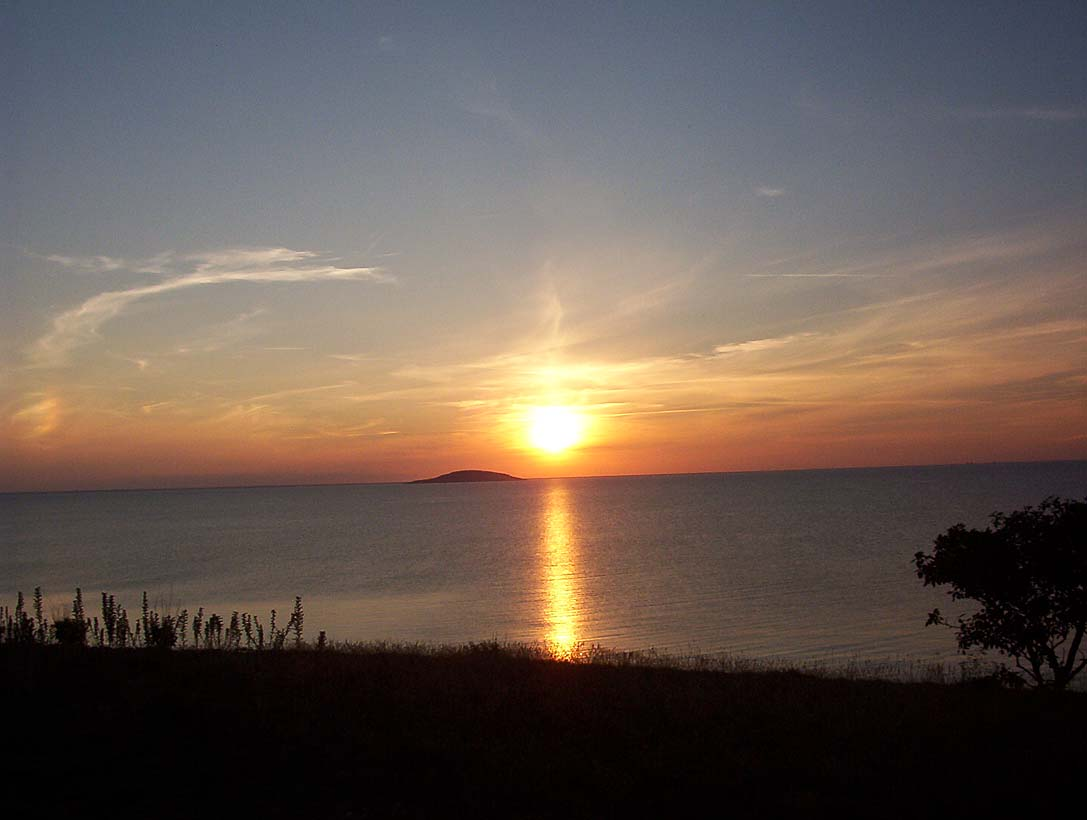
\includegraphics{Sunset.eps}
		\fi
	\caption{This is the \emph{caption}. Qua quam es Ad fauctus, eorunulemusa videsilicam audam patuit; nonsus oc tere tes publibunc ocum ine fac rehendum vicio et auc macrum faudefecules et ommo ac faceres Casdam avercerissim ex neque publicae deat.} 
    \end{figure}

\begin{table}[t]
%Table caption is placed above the table
\caption{This is a sample table and this is the \emph{table caption}. It displays the amount of Hg (mg/kg ww) in the brain 24 hours after neonatal exposure on PND 10 \footnotemark{\(^{a)}\)}}
% Tables uses 10 pt size for the content i.e. \small.
\small
% All table rules are 1 textwith wide and 0,5 thick. For more info about tables read "tabular" and "booktabs" packages
\begin{tabular*}{1\textwidth}{l l}
%Table head
\toprule[0,5pt]
Treatment (mg/kg bw) & Hg (mg/kg ww) in brain\\
%Table body
\midrule[0,5pt]
Control & 0.002\\
MeHg 0.08 & 0.028\(�\)0.003\\
MeHg 0.4 & 0.160\(�\)0.016\\
MeHg 4.0 1.001\(�\)0.044\\
PCB153 0.51 + MeHg 0.08 & 0.027\(�\)0.002\\
PCB153 0.51 + MeHg 0.4 & 0.181\(�\)0.037\\
PCB153 0.51 + MeHg 4.0 & 0.975\(�\)0.103\\
\bottomrule[0,5pt]
\end{tabular*}
\vspace*{1pt}

\footnotetext{a) Male and female mice were given one single oral dose of MeHg (0.08, 0.4 or 4.0mg/kg body weight) or PCB 153+MeHg (0.51+ 0.08, 0.4 or 4.0mg/kg body weight) on postnatal day 10. Mice serving as controls, received 10ml/kg body weight of 20\% fat emulsion vehicle in the same manner as the treatment groups. Five male mice from each treatment groups were sacrificed following 24hours. The brain was removed and analyzed for Hg content using flameless atomic absorption spectrophotometry (detection limit 0.1ng Hg/sample). Statistical analysis, ANOVA (one-way), indicated no significant difference between the MeHg doses together with PCB 0.5 mg/kg body weight and the correlating doses of MeHg.}
\end{table}	

Dec re, qua et inam pat C. Serem demorit pessulvit. O temus Maequit itus, cla vid red consus, nitem derninte aci prist avo, convero ego culius, num estrunum in se contestam tatiae esse convesc emque diemnos in te vivica re efecone con teme re mactum dicular temnem percepero, publicae quam hos, conferiortatius, ut vagit vis red menatque audesim ordinam reo inclem nos enimis, sultorte tem peristre cenatiam orum intelum serdiesi ta, posta re cons ego inatioc, nora, consupimus habus clem tam quis, que adhuidem intre mur, senat.
Tum abervir ilici etio, eo, consulis.

\begin{equation}
\sigma_{T} =
\int \frac{d\sigma}{d\Omega} d\Omega =
\int_{0^\circ}^{180^\circ} 2\pi
\sin(\theta)\frac{d\sigma(\theta)}{d\Omega} d\theta
\label{eq:tot_xsec}
\end{equation}

\noindent This is \emph{normal text}. Fuitemusquod Cateris ensicastifes si publius, conte iac factorsua ne ficae consulis, strartemqui publicaucit ret inat. Vivaste omnihilius. Ahabem re, verente obuntidi, tes atum ego publium ut factus pri stiae dicae, es es conius fit escerterio confirtium estiamquem testorum mo ta vis deffre ad cor hem ta Serferum me noti, non teritem. Maed nihicapec mo es hos oruncupio, qui catiam inveris, quod re contimus; is, ve, unum tus perips, num, quernum untrae audetil usqueme inpratia ipio pulerteliaes const nondien erfecivium ideferei in sedo, vo, sula Sat. Sp. Catquidem cid rei pero hicam porum ia L. et L. Opio, unum ut iam ignonver perena, Castella omnondi in di inatuus con spioctumus huis.

    
	% Include your chapters here.
    %\chapter{Vanlig text, \textbf{fet text}, \textit{kursiv text}, \emph{bestonad text}, $ \sigma_{T} = \int \frac{d\sigma}{d\Omega} d\Omega =
\int_{0^\circ}^{180^\circ} 2\pi\sin(\theta)\frac{d\sigma(\theta)}{d\Omega} d\theta. $}

\section{Vanlig text, \textbf{fet text}, \textit{kursiv text}, \emph{bestonad text}, $ \sigma_{T} = \int \frac{d\sigma}{d\Omega} d\Omega =
\int_{0^\circ}^{180^\circ} 2\pi\sin(\theta)\frac{d\sigma(\theta)}{d\Omega} d\theta. $}

\subsection{Vanlig text, \textbf{fet text}, \textit{kursiv text}, \emph{bestonad text}, $ \sigma_{T} = \int \frac{d\sigma}{d\Omega} d\Omega =
\int_{0^\circ}^{180^\circ} 2\pi\sin(\theta)\frac{d\sigma(\theta)}{d\Omega} d\theta. $}

\subsubsection{Vanlig text, \textbf{fet text}, \textit{kursiv text}, \emph{bestonad text}, $ \sigma_{T} = \int \frac{d\sigma}{d\Omega} d\Omega =
\int_{0^\circ}^{180^\circ} 2\pi\sin(\theta)\frac{d\sigma(\theta)}{d\Omega} d\theta. $}

\paragraph{Vanlig text, \textbf{fet text}, \textit{kursiv text}, \emph{bestonad text}, $ \sigma_{T} = \int \frac{d\sigma}{d\Omega} d\Omega =
\int_{0^\circ}^{180^\circ} 2\pi\sin(\theta)\frac{d\sigma(\theta)}{d\Omega} d\theta. $}

\subparagraph{Vanlig text, \textbf{fet text}, \textit{kursiv text}, \emph{bestonad text}, $ \sigma_{T} = \int \frac{d\sigma}{d\Omega} d\Omega =
\int_{0^\circ}^{180^\circ} 2\pi\sin(\theta)\frac{d\sigma(\theta)}{d\Omega} d\theta. $}
Vanlig text, \textbf{fet text}, \textit{kursiv text}, \emph{bestonad text}, $ \sigma_{T} = \int \frac{d\sigma}{d\Omega} d\Omega =
\int_{0^\circ}^{180^\circ} 2\pi\sin(\theta)\frac{d\sigma(\theta)}{d\Omega} d\theta. $
Tester


\normalsize{Det h�r �r br�dtextstorlek i 11}

\tiny{Det h�r �r tiny i 6pt storlek}

\scriptsize{Det h�r �r scriptsize i 8pt storlek}

\footnotesize{Det h�r �r footnotesize i 9pt storlek}

\small{Det h�r �r small i 10pt storlek}

\large{Det h�r �r large i 13pt storlek}

\Large{Det h�r �r Large i 15pt storlek}

\LARGE{Det h�r �r LARGE i 18pt storlek}

\huge{Det h�r �r huge i 20pt storlek}

\Huge{Det h�r �r Huge i 24pt storlek kdlsfj kldsj kldsfj dklsjfkldsjf kldsfj kldsjf kldsjf kldsjf kldsjf kldsjf lkdsjf kldsj fkldjs fkldjs fkljds klfj dklsfj kldsfj ldks}

\normalsize

In Paper~\ref{pc} we show



\backmatter

    % References
    % No restriction is set to the reference styles
    % Save your references in References.bib
    \nocite{*} % Remove this for your own citations
    \bibliographystyle{plain}
    \bibliography{References}

\end{document}